\section{Réseaux convolutifs}
\label{convsecmain}
\textbf{Important}: Tout ce qui a été vu précédemment s'applique à la spécificité des réseaux convolutifs.
\subsection{Généralités}
Les réseaux convolutifs constituent l'une des grandes familles d'architecture associées aux réseaux de neurones. Popularisés par Yann Lecun en 2012, ces réseaux ont montré des résultats remarquables pour l'analyse de données structurées telles que les images (mais aussi les signaux ou textes). Mais pourquoi cette architecture est préférable à un modèle Feed-Forward (Perceptron Multicouche) standard ?\\

\noindent Supposons une image de petite taille soit 15*15 par exemple. L'image est codée en RGB (images couleurs). Ainsi, l'image possède 15*15*3 valeurs distinctes correspondant à ses pixels. Dans le cas d'un modèle Feed-Forward, les neurones de la couche d'entrée devront avoir une entrée (et donc un poids) associée à chacune des valeurs de l'image soit 15*15*3=675 entrées. Bien que ça puisse impressionner, les capacités de calculs des technologies d'aujourd'hui peuvent le supporter\footnote{Bien sûr, il ne doit pas y avoir trop de couches cachées...}. Considérons une image de taille un peu plus standard soit 500*500. On obtient donc 500*500*3=750*$10^3$ poids par neurones de la couche d'entrée. Il est évident que le nombre d'entrées est bien trop important et rendrait l'apprentissage irréalisable. De même, le risque de sur-apprentissage est très important. De ce fait, les modèles Feed-Forward classique ne \textbf{peuvent pas se mettre à l'échelle}.\\

\noindent Les couches de convolution permettent d'extraire l'information d'une image et d'en réaliser une représentation à un plus haut niveau d'abstraction. Ces couches présentent deux avantages notables. Tout d'abord, elles permettent de représenter le contenu utile d'une image dans une dimension plus faible\footnote{Après traitement d'une couche de pooling} que l'image d'origine\footnote{On peut comparer ce procédé à un pré-traitement des données}, ce qui permettrait à un modèle Feed-Forward d'apprendre dessus. Dans un second temps, les couches de convolution réalisent le travail d'extraction d'information réalisée traditionnellement par des méthodes-tiers comme HoG par exemple et ce, avec une capacité d'apprentissage. Alors que les méthodes-tiers sont des méthodes figées et généralistes, les couches de convolution se spécialisent dans la discrimination des images de sa base d'apprentissage. Ainsi, elles sont souvent plus efficaces et mieux optimisées\footnote{Il a été montré qu'elles offrent une capacité de discrimination assez généraliste dans les couches de bas niveau malgré tout}. Une illustration est visible sur la Figure \ref{absconvpro}\\

\begin{figure}
    \centering
    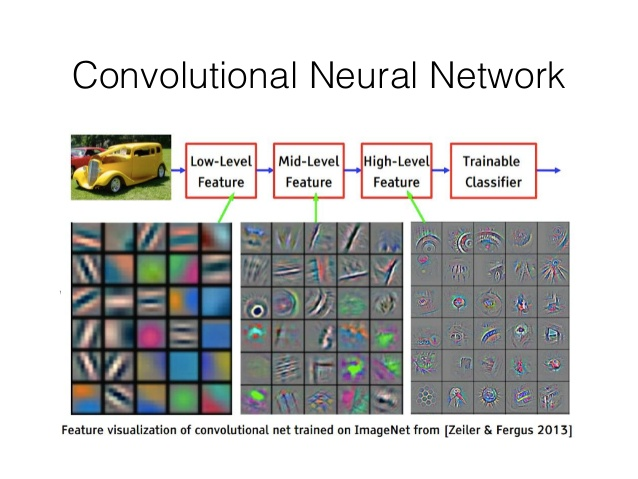
\includegraphics[scale=0.45]{./tex/convolution-network/cnn/convabs.jpg}
    \caption{Relation entre l'abstraction d'un réseau convolutif et sa profondeur}
    \label{absconvpro}
\end{figure}

\noindent Un réseau convolutif possède (dans sa version générale) l'architecture suivante:
\begin{itemize}
    \item \textbf{Couche d'Entrée}: Ceci correspond à la donnée proposée au réseau pour son apprentissage ou une prédiction. L'entrée stocke ainsi l'intégralité des valeurs de la matrice de l'image. Elle sera donc de dimension X*Y*3 dans le cas d'une image de dimension X*Y en RGB.
    \item \textbf{Couche d'extraction de caractéristiques:}\\

    Le cycle suivant est répété k fois en accord avec l'architecture du réseau.
    \begin{enumerate}

    \item \textbf{Couche de convolution}: Les couches de convolution vont extraire l'information de l'image et la représenter à un plus haut niveau d'abstraction. Il peut y avoir une ou plusieurs couches de convolution. La nature des sorties d'une couche de convolution se présente sous la forme d'une matrice de dimension x*y*z où x,y,z dépendant des paramètres de la couche\footnote{x et y inférieurs ou égaux à la dimension X et Y de l'entrée}.

    \item \textbf{Couche d'activation}: Cette couche réalise une activation selon la fonction d'activation utilisée sur les valeurs de la matrice de sortie de la couche de convolution. ReLU est la fonction la plus populaire actuellement mais d'autres peuvent être utilisées.

    \item \textbf{Couche de régulation}: Afin de limiter le sur-apprentissage, il est utile d'exploiter des couches qui aident à prévenir cette dérive de l'apprentissage. Ces couches n'ont pas de pouvoir d'extraction d'informations et se limitent à une action régulatrice. Ce type de couche modifie localement l'architecture du réseau (DropOut par exemple) ou les valeurs de sortie des couches de convolution (Batch Normalisation par exemple).

    \item \textbf{Couche de redimensionnement}: Les sorties des couches de convolution peuvent être dans un format qui ne facilite pas l'apprentissage et/ou l'optimisation de ressources matérielles. Pour limiter ce problème, un redimensionnement vers une dimension inférieure (ou supérieure) est souvent réalisé. Le redimensionnement, selon l'objectif souhaité, s'applique selon une dimension spécifique du signal donné.
    \end{enumerate}

    \item \textbf{Couche de classification (Full-Connected i.e perceptron multicouche)}: Cette couche réalise la décision du réseau à partir de l'information extraite des couches de convolution.
\end{itemize}

\noindent Il est important de noter que certaines couches possèdent des paramètres et d'autres non. En effet, les couches ReLu et Pooling appliquent une transformation fixe sur les données (donc aucun paramètre\footnote{Ceci n'est pas entièrement vrai pour les couches de Pooling car il existe des variantes qui exploitent des paramètres. De même, des variantes plus avancées de la fonction ReLU apprennent durant l'apprentissage}) alors que les couches de convolution et Full-connected "apprennent"\footnote{Par rétro-propagation} durant l'apprentissage et donc, possède des paramètres.

\subsection{Couche d'Entrée}
La couche d'Entrée est représentée par une couche de neurones où un neurone se limite à la propagation d'une valeur de la matrice de l'image observée. Chaque neurone est ainsi défini par une pondération unitaire avec une fonction d'activation linéaire. Il y a autant de neurone que de pixels dans l'image (d'où l'importance d'avoir des images de taille constante).\\

\subsection{Couche de Convolution}

\subsubsection{Nature d'une couche de convolution}

Les couches de convolution suivent une architecture Feed-Forward modifiée par la condition de connectivité locale, i.e un neurone de la couche de convolution n'est pas connecté à l'intégralité des neurones de la couche précédente (Entrée ou autre couche de convolution) mais uniquement aux neurones "les plus proches". Cette particularité diminue drastiquement le nombre de liaison des neurones, permettant leur apprentissage en temps humain. Le degrés de connectivité locale est un paramètre variable dépendant de la taille du filtre souhaité. Un filtre détermine le nombre de neurones adjacents à considérer. Plus le filtre sera grand, plus il y aura de neurones considérés. Néanmoins, bien que la taille du filtre soit variable, sa profondeur reste constante et égale à la profondeur de l'image d'entrée. Par exemple, supposons une image RGB. Sa profondeur est de 3 (channels rouge, vert et bleu). Chaque neurone possédera une connexion avec chacun de ces trois channels en accord avec les limitations du critère de connectivité locale. Il y a donc une restriction selon la largeur et la longueur de la donnée d'entrée mais pas sa profondeur. Une couche de convolution possède un filtre de dimension fixe mais peut posséder plusieurs sous-couches associées à des filtres différents (même dimension mais valeurs différentes). L'architecture d'une couche de convolution se représente donc comme un volume en 3 dimensions où la profondeur correspond au nombre de sous-couches. Une représentation graphique est visible sur la Figure \ref{conv_pic}.\\

\noindent Chaque neurone d'une même sous-couche de convolution possède un même paramétrage. Ainsi, chaque neurone possède le même biais et le même vecteur de pondération. Ils sont donc tous \textit{identiques}. Cette spécificité implique une \textit{invariance par translation} car, comme chaque neurone est identique, la localisation spatiale des pixels n'a pas d'influence sur l'analyse par un filtre donné. De ce fait, une couche de convolution limite grandement le nombre de paramètres tout en conservant les corrélations spatiales locales des images.\\

\noindent Un filtre représente le vecteur poids du neurone. Les poids des neurones ne sont pas identiques pour chaque channel. Ainsi, dans le cas d'une image RGB, un filtre possédera 3 sous-filtres qui seront appliqués sur chacun des channels de manière indépendantes. Les 3 résultats obtenus par les sous-filtres seront unis lors du calcul de la convolution. Dans la configuration standard, on considère souvent un biais nul et une fonction d'activation identité.\\

\noindent Du fait de l'utilisation d'une architecture de neurones, l'apprentissage des filtres se fait par rétro-propagation. Grâce à la connectivité locale du réseau et de l'unicité des pondération par filtre, le nombre de paramètres à apprendre est drastiquement diminué et permet au réseau d'apprendre en temps humain.

\begin{figure}
    \centering
    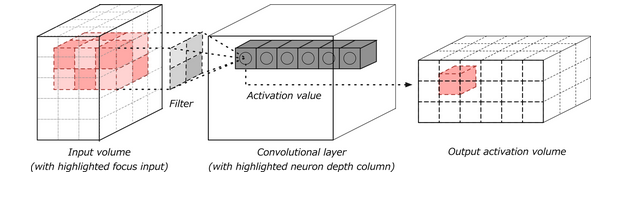
\includegraphics[scale=0.4]{./tex/convolution-network/cnn/conv_fig.png}
    \caption{Architecture d'une couche de convolution}
    \label{conv_pic}
\end{figure}

\subsubsection{Interprétation graphique}
En vulgarisant, une convolution est une opération mathématique qui décrit une règle sur comment unir deux données. Une convolution prend ainsi une entrée, applique un kernel et réalise une \textit{feature map} en sortie.\\

\noindent Dans le cadre d'une couche de convolution, la convolution est réalisée par un produit scalaire entre un filtre (kernel) et l'entrée. Un exemple est visible sur la Figure \ref{conv_fil}. Le filtre est de dimension inférieure à l'entrée (dans le cadre d'une image, inférieure à hauteur*longueur) mais de profondeur égale à la profondeur de l'image (nombre de channels d'entrée). Un filtre se comporte comme une \textit{fenêtre glissante} afin de parcourir l'intégralité de la données d'entrée. La matrice de sortie obtenue est appelée \textit{feature map}. Il y a autant de \textit{feature map} que de filtre ainsi, si il y a 4 filtres appliquées sur la donnée d'entrée, il y aura 4 \textit{feature map} en sortie.\\

\noindent La \textit{fenêtre glissante} est associée à un hyperparamètre appelé \textbf{stride}. En effet, il est possible de définir les intervalles de déplacement. Un stride de 1 implique de réaliser une convolution en appliquant le filtre sur chaque valeur, un stride de deux impliquera un saut de une valeur entre chaque calcul de convolution, etc... Un exemple est visible sur la Figure \ref{stride_fig}. Le stride est très utilisé pour diminuer la dimension des couches de convolution, notamment pour limiter le nombre d'entrée de la couche Feed-Forward qui réalise la décision.\\

\noindent \textbf{Important}: Le kernel est appliqué sur une valeur de la matrice d'entrée en son \textbf{centre}, pas l'un de ses sommets. De plus, un filtre ne réalise la convolution que si chaque élément du filtre s'applique à une valeur de la matrice d'entrée. Observons la Figure \ref{centre_pb}. Sur la représentation de gauche, chaque entité du kernel est associée à une valeur. La convolution peut être définie. A droite, le kernel "dépasse". Le filtre ne peut donc intégralement s'appliquer à la matrice d'entrée: la convolution n'est pas réalisée.\\

\noindent Cette particularité soulève une problématique. Dans cette configuration, la sortie obtenue après convolution ne peut être que de dimension inférieure à l'entrée à cause des effets de bord, effet qui s'aggrave avec des filtres de grandes tailles. Bien qu'une sortie de dimension inférieure ne soit pas un problème en tant que tel (ce serait même bénéfique d'un point de vue temps-machine), elle dénonce une perte d'information de l'entrée sur ses bords. Supposons un kernel de dimension K*K et une entrée D*D, alors la dimension de la sortie sera de dimension (D-K+1)*(D-K+1)\footnote{On supposera un stride de 1}.\\

\noindent Afin de traiter ce problème, la méthode du \textbf{padding} est appliquée. Cette méthode consiste à appliquer une valeur arbitraire et constante afin de combler les valeurs manquantes de la matrice d'entrée. Par convention, la valeur utilisée est 0 (d'où le nom standard de 0-padding\footnote{Parfois, la valeur 1 est employée}). Un exemple est visible sur la Figure \ref{padding}. Cette approche permet de considérer l'information de l'intégralité de la donnée d'entrée et de créer une sortie de même dimension que l'entrée.\\

\noindent Le site Web \url{https://ezyang.github.io/convolution-visualizer/index.html} propose une application intuitive pour visualiser l'impact de différentes configurations sur le comportement des filtres.\\

\noindent En pratique, il faut éviter les filtres de grande taille (5*5, 7*7 et supérieurs) sauf si il y a une vraie pertinence dans le choix de cette échelle de filtre. Les filtre de grande taille sont plus lents à apprendre, gourmand en ressource machine et peuvent être remplacer par des alternatives plus légères avec une efficacité similaire. Il est donc préférable de cumuler des filtres 3*3 dans ce type de cas. Cette approche simple demande moins de paramètres, moins de ressources machine et surtout, plus de non-linéarité.

\begin{figure}
    \centering
    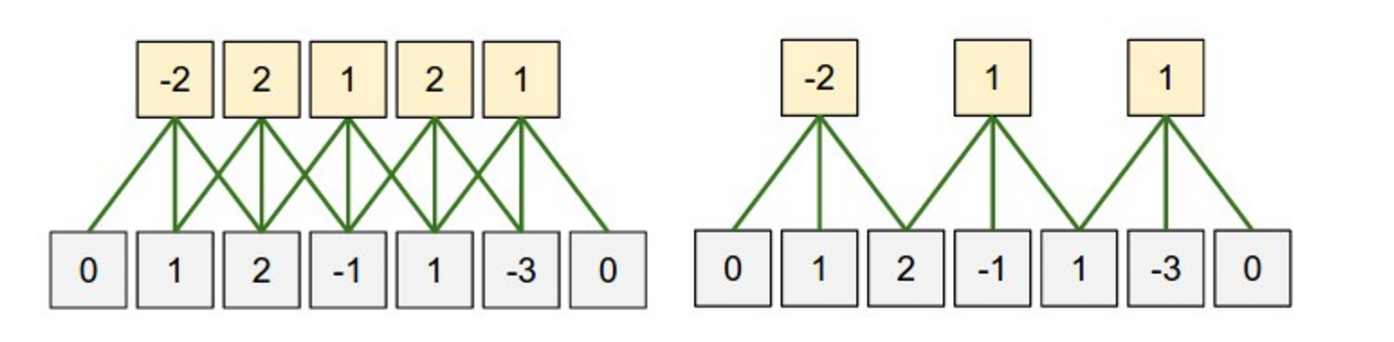
\includegraphics[scale=0.4]{./tex/convolution-network/cnn/stride.png}
    \caption{Impact du stride sur la sortie de la convolution}
    \label{stride_fig}
\end{figure}

\begin{figure}
    \centering
    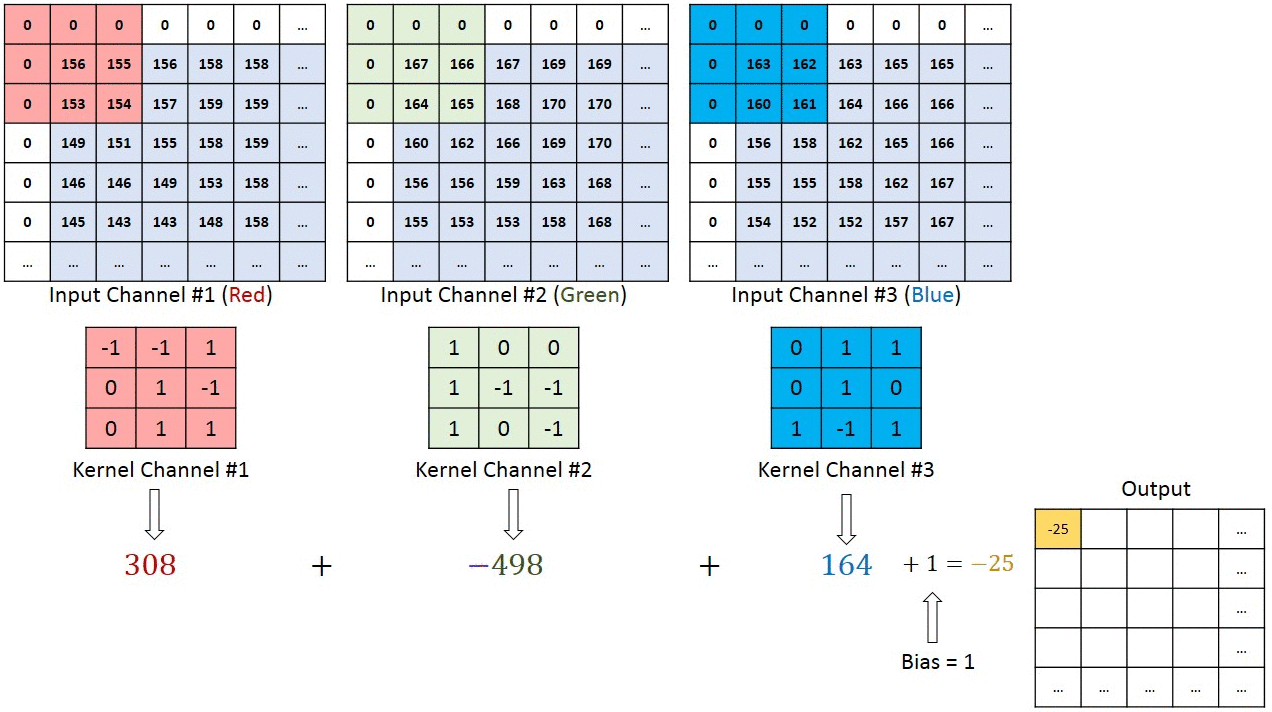
\includegraphics[scale=0.3]{./tex/convolution-network/cnn/conv_filtre.png}
    \caption{Exemple d'une convolution par filtre}
    \label{conv_fil}
\end{figure}

\begin{figure}
    \centering
    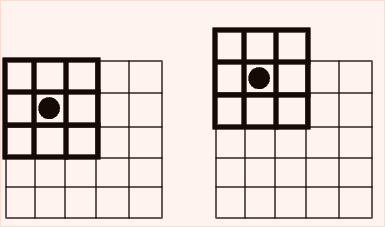
\includegraphics[scale=0.4]{./tex/convolution-network/cnn/padding.png}
    \caption{Problématique de la dimension du filtre: gauche (valide), droite (invalide)}
    \label{centre_pb}
\end{figure}

\begin{figure}
    \centering
    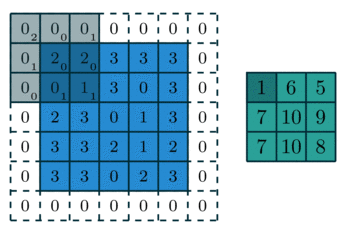
\includegraphics[scale=0.4]{./tex/convolution-network/cnn/padding_.png}
    \caption{Application du 0-Padding}
    \label{padding}
\end{figure}

\subsubsection{Couche de Pooling}
Le \textit{Pooling} est une méthode permettant de compresser (et généraliser) une information locale de la donnée d'entrée. Elle est employée afin de diminuer la dimension des \textit{feature map} tout en conférant une capacité de généralisation à la couche. En effet, le Pooling conserve l'information locale importante, permettant de s'émanciper de détails trop spécifiques (et du bruit).\\

\noindent Le fonctionnement d'une couche de Pooling est comparable à celle d'une couche de convolution si ce n'est qu'elle s'applique sur une \textit{feature map} indépendamment des autres (la profondeur du kernel est de 1). Un filtre (de taille choisie) est appliquée afin de définir \textit{l'environnement local}\footnote{Comparable à une isolation spatiale} et un opérateur est appliqué sur les valeurs d'entrée ciblées par le filtre. La nature de cet opérateur est variable: Max, Average\footnote{Ces deux opérateurs sont les plus fréquents}. Expérimentalement, la fonction Max est la plus utilisée. Sur la Figure \ref{maxpool_fig}, nous pouvons observer l'application d'un Max-Pooling de filtre 2*2.\\

\noindent \textbf{Remarque}: Le Pooling doit être exploitée avec parcimonie. Il est souvent un \textit{bottleneck} pour la vélocité du modèle. De même, son utilisation ne fait pas l'unanimité dans le milieu scientifique. En effet, Geoffrey Hinton, chercheur de renom dans le domaine de l'apprentissage profond, a déclaré: "\textit{The pooling operation used in convolutional neural networks is a big mistake and the fact that it works so well is a disaster."} (Reddit AMA).\\

\noindent Ce scepticisme repose sur plusieurs défauts de cette approche. Le Pooling est une action non évolutive (fixe donc sans apprentissage), ce qui nuit à la capacité de généralisation/spécialisation. De plus, son action est locale à une \textit{feature map}. Il y a donc une perte importante d'informations associées aux relation inter-feature map. Pour finir, le Pooling a une capacité explicative lorsque les couches de convolutions présentent un fort taux d'abstraction. Dans le cas contraire, le filtre est souvent de taille trop faible pour considérer une information discriminante. Augmenter la taille du filtre est envisageable mais le Pooling étant \textit{destructeur}, l'augmentation du filtre aurait des conséquences désastreuses sur la transmission de l'information aux couches supérieures.\\

\noindent Plus récemment, des propositions de fonctions de Pooling ont été faites. Nous pouvons citer:
\begin{itemize}
    \item \textbf{$L_p$ Pooling}\cite{lppool}: Cette approche est issue des études biologiques des cellules vivantes. Elle est définie par: $y_{m,n,k}=\left[\sum_{(i,j) \in R_{mn}} (a_{i,j,k})^p \right]^{\frac{1}{p}}$ avec $R_{mn}$, surface du filtre et k, channel analysé.\\

    Il s'agit de la norme $L_p$ des valeurs ciblées par le filtre du Pooling. Ainsi, si p=1 alors $L_p$ correspond à l'average Pooling. Si $p= \infty$, $L_p$ correspond au max Pooling. Cette méthode permet de réaliser un compromis entre l'isolation discriminante d'une information et la généralisation du message locale.

    \item \textbf{Mixed Pooling}\cite{mixedpool}: Cette méthode combine max Pooling et average Pooling au sein d'une combinaison linéaire dont les coefficients pondérateurs dépendent d'un paramètre $\lambda$ tel que $\lambda \in \mathcal{U}(0,1)$. Ainsi, nous obtenons: $$y_{m,n,k}=\lambda \  max_{R_{mn}}a_{i,j,k}+(1-\lambda)\frac{1}{|R_{mn}|}\sum_{(i,j)\in R_{mn}}a_{i,j,k}$$

    Expérimentalement, elle présenterait de meilleurs résultats que l'approche max ou average tout en proposant une plus grande résistance au sur-apprentissage.

    \item \textbf{Gated max-average Pooling}\cite{mixedpool}: Cette approche est similaire à \textit{Mixed Pooling} mais considère l'état de la surface couverte par le Pooling. En effet, \textit{Mixed Pooling} applique un coefficient indépendamment des valeurs couvertes par le filtre de Pooling. \textit{Gated max-average Pooling}, au contraire, va réaliser une pondération évolutive selon les valeurs couvertes par le filtre. On suppose x, valeurs couvertes par le filtre de Pooling et w, "Gate" du Pooling. Cette idée est traduite par:

    $$ f_{gate}=\sigma(w^Tx)f_{max}(x)+(1-\sigma(w^Tx))f_{avg}(x)$$
    $$\sigma(w^Tx)=\frac{1}{(1+exp(-w^Tx))} $$

    La "Gate" peut être unique à un réseau, une couche, à une région de la couche mais identique sur toute la profondeur ou au contraire, différente sur toutes les profondeurs. Néanmoins, cela ajoute des paramètres à apprendre et donc un ralentissement de la vitesse d'apprentissage. Cette approche présente des résultats plus performants que \textit{Mixed Pooling}.

    \item \textbf{Stochastic Pooling}\cite{stopool}: Cette méthode choisit une valeur selon une distribution de probabilité définie par $p_i=\frac{a_{i}}{\sum_{k \in R_{mn}}a_k}$ avec $i \in [1, |R_{mn}|]$ et $R_{mn}$, l'ensemble des valeurs isolées par le filtre du Pooling.\\

    Ainsi, plus une valeur est élevée, plus la chance d'être choisie est importante. Cette méthode permet de limiter le sur-apprentissage comparée au max-Pooling en introduisant un comportement probabiliste sur la sélection de la valeur.\\
\end{itemize}
\begin{figure}
\begin{tabular}{cc}
    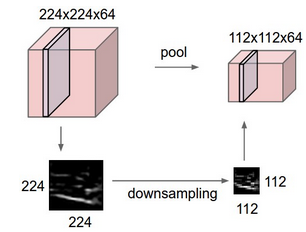
\includegraphics[scale=0.4]{./tex/convolution-network/cnn/pooling_ex.png}  & 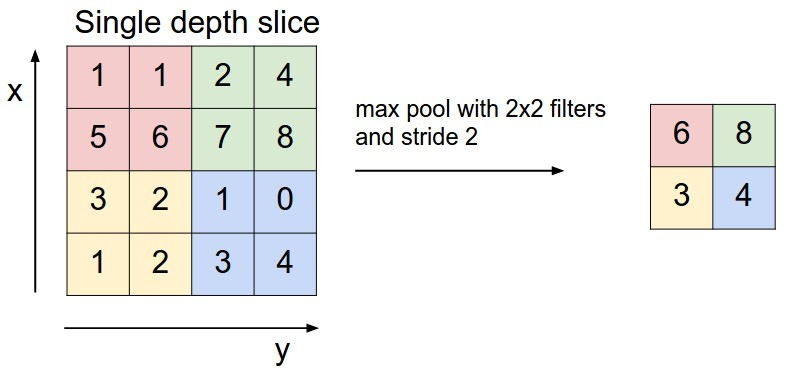
\includegraphics[scale=0.3]{./tex/convolution-network/cnn/maxpool.jpeg} \\
\end{tabular}
\caption{Application du Pooling: Réduction et exemple avec la fonction max selon un filtre 2*2}
\label{maxpool_fig}
\end{figure}

\noindent \textbf{Remarque}: Dans les faits, ces méthodes de Pooling sont assez marginales et peu exploitées. L'écrasante majorité des réseaux actuels exploitant des approches par Pooling reposent sur l'opérateur Max ou Average.\\

\noindent L'opérateur Max est utile lorsque l'on cherche à extraire une information discriminante au détriment des autres. L'objectif est d'isoler les éléments les plus discriminants afin de les analyser par la suite (notamment par un réseau Full-Connected). Cette approche est très utile pour la classification d'images par exemple. En effet, pour classer, un élément discriminant est nécessaire et suffisant. D'autres données moins informatives risqueraient de se comporter comme une forme de bruit.\\

\noindent L'opérateur Average ne se focalise pas sur les élements discriminants du signal mais sur son comportement général. Sa valeur est donc un résumé global de ses caractéristiques et non d'un aspect discriminant spécifique. Cet opérateur est donc moins destructeur mais possède un pouvoir discriminant plus faible.\\

\noindent La couche de Pooling, selon la configuration, peut conserver des informations utiles pour d'autres couches. Par exemple, dans le cas du Max-Pooling, une mémorisation de la localisation de la valeur max sur la matrice de données peut être réalisée. Cette information permet de réaliser des mises à l'échelle (via Unpooling) avec plus de fidélité mais demande de la mémoire pour stocker les valeurs.\\

\noindent \textbf{Remarque}: Expérimentalement, on a tendance à éviter le chevauchement des filtres de Pooling. Ainsi, on exploite un stride en édéquation avec la dimension du kernel pour que chaque valeur de la \textit{feature map} soit analysée une unique fois. Par exemple, dans le cadre d'un kernel 2*2, on aura tendance à utiliser un stride de 2.

\paragraph{Global Pooling}

\noindent Global Pooling est l'équivalent du pooling mais son application n'est pas limitée par la fenêtre correspondant à la taille du filtre. Il ne s'effectue donc pas sur un sous-ensemble (défini par le filtre) d'une \textit{feature map} mais sur l'intégralité d'une \textit{feature map}. Une \textit{feature map} est donc représentée par une unique valeur à l'issu d'un Global Pooling.  Ainsi, supposons une donnée de la forme 15*15*3 avec 3, profondeur\footnote{Nombre de \textit{feature map} présents dans la sortie considérée} de la sortie. La sortie sera donc représentée par un vecteur de dimension dans $R^3$.\\

\noindent Le Global Pooling est une méthode utilisée pour lutter contre le sur-apprentissage et  diminuer le volume des calculs des réseaux convolutifs, notamment de la couche Full-connected réalisant la classification. Les capacités de régulation du Global Pooling s'expriment sous différents aspects:

\begin{itemize}
    \item \textbf{Sans apprentissage}: Étant donné que le Global Pooling considère l'intégralité d'une \textit{feature map}, il n'y a pas d'apprentissage associée à cette couche, ce qui n'ajoute pas de temps d'apprentissage

    \item \textbf{Optimisation de la relation Label - Feature Map}: La couche de Full-connected réalise la prédiction à partir des \textit{feature map}. Les \textit{feature map} sont donc les porteuses d'informations qui doivent retranscrire les spécificités d'un label (catégorie). Il existe un risque important que les feature maps "brutes" soient trop spécifiques du fait des dimensions matricielles élevées de leurs structures, ce qui provoque des dérives vers le sur-apprentissage. L'approche du Global Pooling, en limitant à une valeur par \textit{feature map}, favorise la correspondance entre une \textit{feature map} et une caractéristique générale.

    \item \textbf{Généralisation Spatiale}: En résumant une \textit{feature map} à une valeur, le Global Pooling permet de généraliser l'information. Cette méthode permet donc d'extraire une caractéristique indépendamment de considérations spécifiques due à l'image d'entraînement telles que l'angle de vue, le contraste ou encore la luminosité par exemple.

    \item \textbf{Temps d'apprentissage}: Le Global Pooling limite grandement le nombre de valeurs d'entrée de la couche Full-connected. Cette méthode permet donc d'en diminuer la taille, ce qui rendra le modèle plus rapide à apprendre, à calculer ses prédictions et plus léger d'un point de vue mémoire.
\end{itemize}

\noindent Le Global Pooling est une approche de plus en plus utilisée pour réaliser la liaison entre l'ensemble des couches de convolution et le réseau Full-Connected, remplaçant ainsi la méthode dite \textit{Flatten} classique qui consiste à vectoriser les features map dans leur intégralité. Néanmoins, Global Pooling est très destructeur et présente des faiblesses notamment dans le cas de données textuelles (classification de textes par réseau convolutif par exemple).

\paragraph{k-Max Pooling}
Afin de corriger le comportement destructeur du Global Pooling, k-Max Pooling\cite{kmaxpool} applique l'opérateur pour conserver les k valeurs\footnote{Si k est égal à 1, le comportement est identique à un Global Max Pooling} les plus importantes (au lieu d'une seule pour le Global Pooling). Du fait d'un résultat non unitaire, l'opérateur Average n'est pas exploitable par cette approche.\\

\noindent Le choix de la valeur de k peut être difficile à réaliser. Une valeur trop faible posséderait les mêmes faiblesses qu'un Global Max Pooling et une valeur trop élevée nuirait à la capacité de généralisation recherchée par l'exploitation de ce type de couche. De plus, comme le Pooling s'exerce sur une \textit{feature map} uniquement, la profondeur est à considérer lors du choix de la valeur de k. En effet, en supposant n \textit{feature map} en entrée, la sortie de la couche de k-Max Pooling sera de dimension $n*k$.\\

\noindent Les couches de convolution permettent d'extraire l'information utile d'un signal. Néanmoins, elles sont directement dépendantes de la qualité de la donnée en entrée. Une donnée trop bruitée provoquera un résultat médiocre peu importe la qualité du modèle employé. Une couche de Pooling mal exploitée peut être une source de contre-performance du réseau du fait de son grand pouvoir destructeur. Il est donc intuitif de penser que dans un réseau qui cumule plusieurs couches de Pooling, le pouvoir généralisant doit être progressivement exploité pour ne pas perdre d'informations en amont des couches convolutives. En d'autres mots, dans le cadre du k-Max Pooling, k doit avoir une valeur plus importante au niveau des couches basses et une valeur plus faible au niveau des couches élevées.\\

\noindent Pour répondre à cette problématique, Dynamic K-Max Pooling \cite{kmaxpool} a été proposé. Cette approche propose une détermination automatique de la valeur de k en fonction de l'architecture du réseau et de la position de la couche de Pooling dans ce dernier.\\

\noindent La valeur de k est définie par: $k_l=max(k_{top},\lceil\frac{L-l}{L}*s\rceil)$ avec $k_{top}$, valeur minimale de k pour les couches supérieures, L, nombre total de couches de convolution dans le réseau, l, position de la couche où le Pooling est appliqué et s, dimension\footnote{A l'origine, cette approche de Pooling a été proposée pour l'analyse de texte. De ce fait, s correspond à la dimension du texte en entrée. Il est possible de généraliser à un signal 2D comme un image mais il est probable que la fonction doive être modifiée pour mieux correspondre aux caractéristiques d'une image} de la \textit{feature map}.\\

\noindent La fonction proposée permet d'avoir une diminution progressive de la valeur de k (jusqu'au seuil critique $k_{top}$ et ainsi, d'augmenter le pouvoir discriminant des couches de Pooling en adéquation avec les caractéristiques informatives des données entrantes. La fonction proposée par \cite{kmaxpool} est "arbitraire" et ne repose sur aucune véritable justification mathématique si ce n'est l'intuition des auteurs. Elle peut être modifiée afin d'obtenir un comportement plus spécifique sur la vitesse de décroissance. De plus, elle est spécifique à une donnée textuelle. Dans le cadre d'une image, il est pertinent d'envisager une autre fonction qui sera en adéquation avec le comportement d'un signal 2D.

\subsubsection{Couche de Unpooling}
Le Unpooling est une approche de \textit{Upsampling}, i.e l'augmentation de la dimension de représentation d'une données. Cette approche est utilisée après une une couche de pooling lorsqu'une mise à l'échelle est nécessaire. Elle exploite la capacité de la couche de pooling à conserver des informations de position\footnote{Dans le cas de l'average-pooling, ce n'est pas nécessaire} (notamment pour Max-Pooling). La configuration de la \textit{feature map} de sortie dépend de la méthode de pooling choisie. Ainsi, dans le cas d'un max-pooling, seule la valeur à la position correspondant à la position de la valeur max sur la donnée d'entrée (bornée par la surface couverte par le filtre) sera définie, les autres valeurs étant considérées comme 0. Une illustration est visible sur la Figure \ref{unpooling}. \\

\begin{figure}
    \centering
    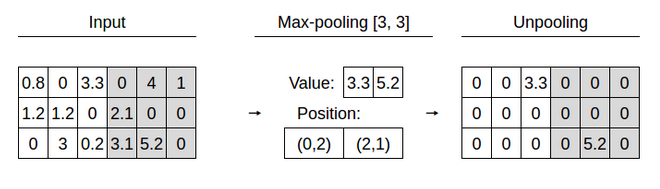
\includegraphics[scale=0.4]{./tex/convolution-network/cnn/unpooling2.png}
    \caption{Exemple de Max-Unpooling statique}
    \label{unpooling}
\end{figure}

\noindent L'exemple présenté est statique (réutilise les valeurs max sans apprentissage). Une approche similaire consiste à ne pas utiliser la valeur max de la \textit{feature map} d'entrée et à appliquer un autre filtre, entraînable, afin de définir les valeurs de la nouvelle \textit{feature map}. De ce fait, seules les informations de position sont utilisées. Un exemple est visible sur la Figure \ref{unpooling2}.

\begin{figure}
    \centering
    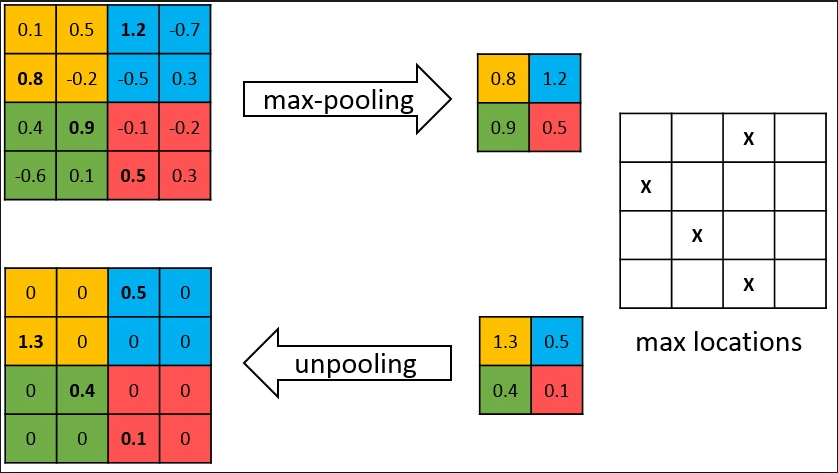
\includegraphics[scale=0.3]{./tex/convolution-network/cnn/unpooling.png}
    \caption{Exemple de Max-Unpooling dynamique}
    \label{unpooling2}
\end{figure}

\subsubsection{Couche de convolution 1*1}
Un cas particulier est la couche de convolution 1*1. Au premier regard, cette convolution semble non pertinente voire sans intérêt\footnote{Pour les lecteurs sensibilisés au traitement du signal, c'est un quasi non-sens}. Néanmoins, du fait de la considération obligatoire de la profondeur de la donnée d'entrée, ce type de convolution possède un intérêt certain. En effet, elle a la capacité de modifier la profondeur de sortie de la couche de convolution où la profondeur correspondra au nombre de filtre présent dans la couche de convolution 1*1. Supposons une donnée d'entrée de dimension X*Y*Z avec Z, profondeur de cette donnée. L'application d'une couche de convolution 1*1 avec N filtres créera une sortie de dimension X*Y*N. Cette méthode complète l'approche par pooling. En effet, le pooling limite la dimension de la \textit{feature map} et la convolution 1*1 limite la profondeur de sortie, i.e le nombre de \textit{feature map}. \\

\noindent Cette convolution ne se focalise que sur la valeur ciblée par le filtre sans considération des corrélations locales mais tient compte de l'ensemble des channels de la donnée d'entrée\footnote{La profondeur est toujours considérée dans son intégralité}. Elle permet donc d'ajouter de la non-linéarité dans l'architecture du réseau\footnote{Ce qui est souvent favorable aux performances du réseau}.

\subsubsection{Couche de convolution dilatée}
Les couches de convolution dilatées\cite{dilate} introduisent un nouveau paramètre: \textbf{le taux de dilatation}. Le taux de dilatation détermine l'espace entre chaque valeur effective du kernel. Par exemple, un kernel 3*3 avec un taux de dilatation de 2 deviendra un kernel de 5*5 car le filtre ne se focalisera pas sur des éléments adjacents $a_i$, $a_{i+1}$ mais sur des éléments distants en accord avec le taux de dilatation. Ainsi, pour une dilatation de 2, les éléments ciblés seront $a_i$, $a_{i+2}$. Les valeurs contenues dans le champ réceptif mais non effectives auront une valeur imposée à 0 (car le poids associé sera nul). La Figure \ref{dilate} illustre ce type de convolution.\\

\noindent Cette approche permet d'élargir le champ d'analyse de la couche en conservant le même coût de calcul. Elle est très utilisée pour la détection d'entités ou la segmentation car elle offre un bon compromis de performance. Elle permet une analyse générale d'une image sans multiplier les convolutions ou l'utilisation de filtres larges qui sont très gourmands en ressources. Par exemple, supposons un filtre 3*3 (stride 1) classique. En combinant 3 couches composées de ce filtre, le champ réceptif de la dernière couche sera de 7*7 ($3*3 \rightarrow 5*5 \rightarrow 7*7$). Au contraire, avec une dilatation de 2, la surface couverte sera de $15*15$.

\begin{figure}
    \centering
    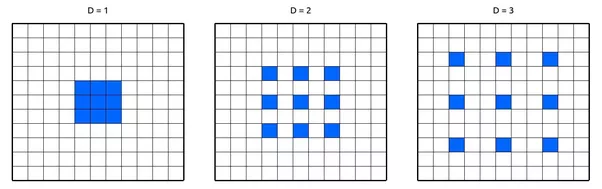
\includegraphics[scale=0.4]{./tex/convolution-network/cnn/dilated.png}
    \caption{Exemple d'une convolution dilatée}
    \label{dilate}
\end{figure}

\subsubsection{Couche de convolution transposée}
\textbf{Remarque}: Cette couche est aussi appelée \textit{fractionally strided convolutions} ou \textit{déconvolution}. L'appellation "déconvolution" est un abus de langage. Cette couche ne réalise pas une déconvolution au sens mathématique du terme.\\

\noindent Une couche de convolution transposée a pour objectif de mettre à une dimension \textbf{supérieure} choisie, une donnée d'entrée. Il s'agit ainsi d'une technique de \textit{Upsampling}. C'est très utilisé en segmentation afin de mettre à l'échelle la sortie d'un réseau convolutif.\\

\noindent Son fonctionnement est comparable à une convolution standard avec l'application de padding (ajout de 0 arbitraire) afin de compléter la donnée d'entrée et mettre à l'échelle voulue la \textit{feature map} de sortie. Le padding dépend de la taille du filtre choisie, du stride et de la dimension de sortie du \textit{feature map}. Deux exemples sont visibles sur la Figure \ref{local_fig}.\\

\noindent Les couches de convolution transposées permettent uniquement de conserver les dimensions des features map. Ainsi, supposons une entrée N alors l'application d'une couche de convolution sur cette entrée puis d'une couche de déconvolution (avec le même paramétrage de couche que la couche de convolution) permettra d'obtenir une sortie de même dimension que N. Par contre, la sortie n'est \textbf{pas égale} à N ! D'où l'abus de la dénomination \textit{déconvolution} qui est faux mathématiquement parlant.

\begin{figure}
\centering
\begin{tabular}{cc}
    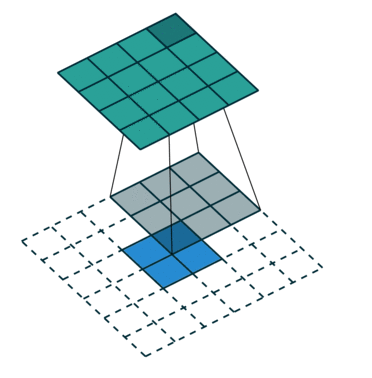
\includegraphics[scale=0.4]{./tex/convolution-network/cnn/transposed.png}  & 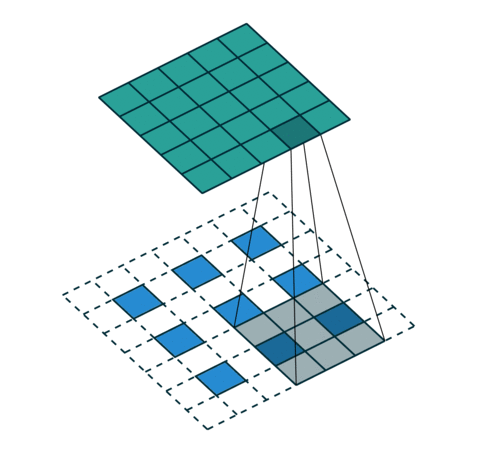
\includegraphics[scale=0.4]{./tex/convolution-network/cnn/transpose2.png} \\
\end{tabular}
\caption{Exemple de convolution transposée: Gauche: entrée 2*2 sans stride, Droite: Entrée 3*3 avec stride de 1}
\label{local_fig}
\end{figure}

\subsubsection{Couche de Depthwise/Pointwise}
\label{depthwiseconv}
Bien qu'efficaces, les couche de convolution standards restent gourmandes en temps de calcul et en mémoire nécessaire pour stocker le modèle. Dans des contextes particuliers avec des limitations de ressources tels que l'embarqué ou encore les smartphones/tablettes, l'utilisation de modèle très profond classique n'est pas envisageable pour cause de limitation matérielle. En plus des méthodes standards de réduction vues dans les Sections précédentes, il est possible d'agir au niveau de l'architecture-même des couches de convolutions avec les couches de \textbf{Depthwise/Pointwise} (ou separable depthwise). Ce type de couche a été popularisé par la création de l'architecture \textit{MobileNet}\cite{mobilenet} crée par Google afin de répondre aux problématiques des prédictions sur smartphone. \\

\noindent Le comportement général de ce type de couche est comparable aux couches de convolution standards. La différence se situe au niveau des spécificités du nombre de filtres et de leurs dimensions. Une couche de depthwise/pointwise se découpe en deux parties: la partie depthwise et la partie pointwise. La couche depthwise est comparable à une couche de convolution standard mais avec \textbf{uniquement} un filtre. Dans une couche de convolution depthwise/pointwise, il n'y a qu'une couche depthwise. La couche pointwise est comparable à une couche de convolution standard avec un filtre de dimension \textbf{1*1} et s'applique sur la sortie \textit{intermédiaire}\footnote{Avant l'étape d'addition par rapport à une convolution standard} de la couche depthwise. Cette couche peut être cumulée N fois. Une illustration de cette couche est visible sur la Figure \ref{depthwise_fig}.\\

\begin{figure}
    \centering
    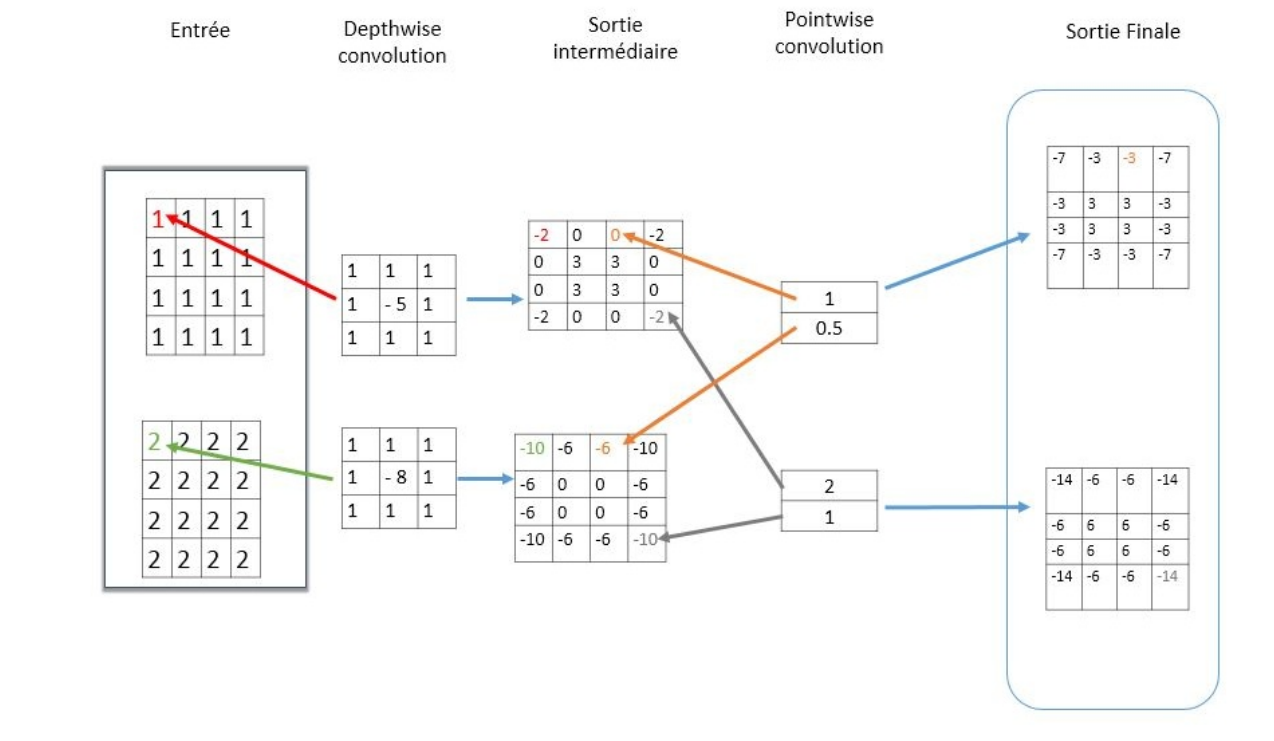
\includegraphics[scale=0.3]{./tex/convolution-network/cnn/depthwise.png}
    \caption{Exemple d'une couche Depthwise/Pointwise avec 2 filtres}
    \label{depthwise_fig}
\end{figure}

\noindent Étudions dorénavant les bénéfices de ce type d'approche. Supposons une entrée (matrice carrée) de dimension X*X*M avec M, profondeur de l'entrée. On lui applique N filtres (composés de sous-filtres en accord avec la profondeur de la donnée d'entrée). On supposera que chaque filtre possède une dimension identique de taille K*K. Le coût de calcul d'une couche de convolution standard est donc de (X*X)*M*(K*K)*N\footnote{On suppose un stride de 1 et un 0-padding nécessaire pour conserver la même dimension entre les données d'entrée et la \textit{feature map} de sortie}.\\

\noindent Considérons maintenant une couche depthwise/poitnwise. On a alors:

$$D_{depthwise/poitnwise}=D_{depthwise}+D_{pointwise}$$
$$D_{depthwise}=(X*X)*M*(K*K)*1$$
$$D_{pointwise}=(X*X)*M*(1*1)*N$$
$$D_{depthwise/poitnwise}=(X*X)*M*(K*K)*1+(X*X)*M*(1*1)*N$$
~~\\
La différence de coût de calcul est donc définie par: $$\frac{(X*X)*M*(K*K)*1+(X*X)*M*(1*1)*N}{X*X)*M*(K*K)*N}=\frac{1}{N}+\frac{1}{K^2}$$
~~\\
Ce résultat permet d'évaluer la pertinence de ce type de couche. En effet, on peut observer que plus le nombre de couche est importante (N) et/ou la taille du filtre grand (K), plus l'économie en temps de calcul est important. Cette économie est associée au temps de calcul machine et au temps d'apprentissage, le rapport étant identique pour les deux économies. Ainsi, pour les réseaux très profonds sur des supports de faible puissance, cette approche propose une solution performante.\\

\noindent Néanmoins, cette approche donne des résultats moins performants bien que ce défaut soit négligeable face au temps machine et d'apprentissage. L'utilisation ou non de ce type de couche relève des spécificités du problème à résoudre. Il est intéressant de noter que cette approche a été très sollicitée (et avec succès) sur les supports mobiles comme les smartphones.

\subsection{Conversion d'une couche Full-Connected en couche de convolution}
\label{convfctoconv}
Une couche Full-Connected, par un "jeu de couches", peut être remplacée par une approche exclusivement convolutive. Bien que cette approche puisse sembler \textit{tricky}, elle est très utile afin d'optimiser certains réseaux qui exigent un calcul de prédiction rapide en limitant la redondance de calcul (algorithmes de \textit{Tracking} par exemple).\\

\noindent Observons la Figure \ref{fulltoconv}. En haut, un réseau convolutif classique avec deux couches Full-Connected en fin de réseau finalisées par un \textit{Softmax}. Une sortie \textit{Softmax} est caractérisée par une couche composée de neurones comportant autant de sortie que de classes discriminées suivie d'une activation par une fonction \textit{Softmax}. Dans notre exemple, supposons que le réseau discrimines 4 classes, i.e 4 neurones sur la couche de sortie.\\

\noindent La première couche de Full-Connected est connectée à une sortie de dimension 5*5*16. Un neurone possède donc 5*5*16 entrées distinctes. Observons le réseau entièrement convolutif (réseau du bas sur la Figure \ref{fulltoconv}). La couche Full-Connected est remplacée par une couche convolutive de kernel 5*5 et de profondeur 400. La sortie de cette couche sera donc de dimension 1*1*400. Cette couche de convolution est donc déterminée par 400 neurones où seul un neurone caractérise un filtre. Un kernel, par convention, s'applique sur toute la profondeur. Ainsi, chaque neurone de la couche de convolution reçoit 5*5*16 (hauteur*largeur*profondeur) valeurs pondérées par des poids distincts (et apprenants). Par conséquent, ces deux architectures sont mathématiquement identiques car le logit formé est issu d'une relation linéaire similaire et la couche présente autant de neurones.\\

\noindent Afin de réaliser la conversion, il faut donc créer une couche de convolution dont la dimension du kernel est égale à la dimension (hauteur et largeur) des features map en entrée. Le nombre de filtre de cette couche de convolution est égale au nombre de neurones de la couche Full-Connected.

\begin{figure}
    \centering
    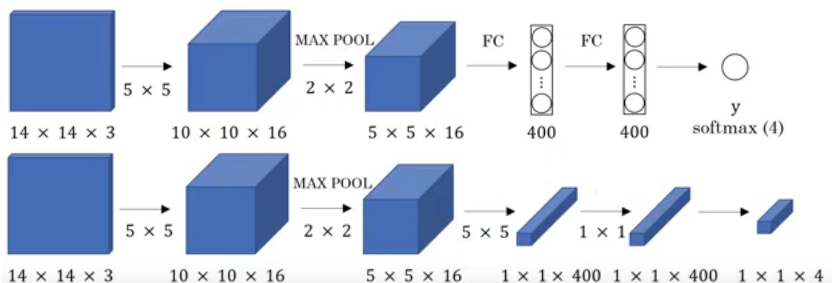
\includegraphics[scale=0.4]{./tex/convolution-network/cnn/fctoconv1.png}
    \caption{Exemple d'une conversion de couche Full-Connected vers une structure convolutive}
    \label{fulltoconv}
\end{figure}

\subsection{Convolutional Neural Network (CNN) et Fully Convolutional Network (FCN)}
Avec l'évolution de la Recherche, une famille d'architecture a été crée: \textit{Fully Convolutional Network}\cite{fcn} (FCN).\\

\noindent Contrairement à l'architecture CNN standard, FCN n'utilise pas de couche Full-Connected mais exclusivement des couches convolutives\footnote{D'où le nom Fully Convolutional Network}. La prise de décision du réseau est donc assurée par des couches convolutives tout comme l'extraction d'attributs.\\

\noindent Un réseau FCN va donc essayer d'extraire les informations et de prendre une décision selon des données \textbf{spatialement indépendante} du fait de l'isolation réalisée par le fonctionnement de la convolution. Chaque \textit{sous-décision} de la couche convolutive est basée sur l'information isolée par la taille du filtre. Au contraire, CNN aura tendance à considérer l'information dans sa \textbf{globalité} du fait de l'utilisation de couches Full-Connected qui exploite intégralement les données. Il n'y a donc pas de considération de \textit{localité}. Ces dernières années, les réseaux FCN gagnent en popularité du fait de leur efficacité similaire et de leur plus grande vitesse d'apprentissage. De même, un FCN permet une plus grande robustesse face à des données de dimensions variables\footnote{Les couches Full-Connected sont dépendantes de la dimension de la donnée d'entrée} tout en réalisant la conversion d'échelle plus rapidement.

\subsection{Les modèles convolutifs de référence}

\subsubsection{AlexNet}
AlexNet\cite{alexnet}(2012) est une référence historique du Deep Learning. Il est le modèle précurseur des architectures convolutives (reposant sur l'architecture LeNet développée par Lecun) et a présenté des résultats remarquables en gagnant le 2012 ILSVRC\footnote{Il s'agit d'une des compétions - voire la compétition - la plus prestigieuse et compétitive de vision par ordinateur} (ImageNet Large-Scale Visual Recognition Challenge) avec 10\% d'erreur en moins que le 2nd. Il constitue un cas d'école pertinent pour apprendre les fondations d'un réseau convolutif (couche de convolution, max-pooling, dropout, ReLu...) et a été défini pour classer 1000 catégories au plus. Du fait de son ancienneté, il tend à devenir "obsolète" aujourd'hui.

\subsubsection{ZF Net}
ZF Net\cite{zfnet}(2013) est un modèle basé sur AlexNet et vainqueur du 2013 ILSVRC. La différence majeure se situe sur la taille des filtres, notamment des premières couches. L'idée derrière cette réduction était de limiter un maximum la perte d'information associée à un filtre trop grand (trop généraliste) de la donnée initiale. De plus, il n'a été entraîné que sur 1.3 million d'image et non 15 milions comme AlexNet.\\

\noindent L'apport majeur de ce modèle (et du papier de recherche associé) est la méthode de visualisation DeConvNet (Deconvolutional Network). Cette méthode permet d'examiner les caractéristiques d'activation des différentes couches et d'offrir un aperçu de ce que "voit" et discrimine la couche observée. Cette architecture a permis de mieux comprendre le comportement interne des réseaux convolutifs et leurs critères de discrimination\footnote{On est encore loin de comprendre parfaitement le fonctionnement des réseaux neuronaux. C'est toujours un sujet de recherche très intense et d'une nécessité prioritaire}. On le nomme DeConvNet du fait de l'inversion de la transformation réalisée. Au lieu de passer de "pixels à map feature", ce réseau passe de "map feature à pixels".

\subsubsection{VGG Net}
VGG Net\cite{vggnet}(2014) est un finaliste (mais perdant) de 2014 ILSVRC. Ce réseau exploite une architecture "simple" mais profonde. En effet, ce modèle se limite à cumuler des couches de convolution utilisant des filtres 3*3 - stride 1 et des couches de max-pooling 2*2 - stride 2. La contribution principale de ce modèle a été de montrer que la profondeur est un composant critique de bonne performance. Néanmoins, c'est un modèle lourd (en ressources matérielles et paramètres) bien qu'il puisse être grandement simplifié en supprimant des couches de Full-connected sans une perte significative de performance. Il s'agit d'un modèle encore très utilisé aujourd'hui.

\subsubsection{GoogleNet/Inception}
GoogleNet\cite{googlenet}(2014) est le vainqueur du 2014 ILSVRC. L'architecture de ce modèle est très novatrice (elle s'inspire, néanmoins, de l'approche Network in Network\cite{nin})\footnote{Nous n'aborderons pas ce papier. Il a une importance théorique mais n'apporte pas d'élément applicatif concret dans le cadre de ce cours}. Elle s'oppose au dogme du modèle séquentiel (succession de couches à flux unitaire) et propose une approche en "largeur" (en parallèle). Ce modèle a ainsi proposé une nouvelle forme de \textit{block}: \textbf{l'Inception module}. Sa structure est représentée sur la Figure \ref{inception}.\\

\begin{figure}
    \centering
    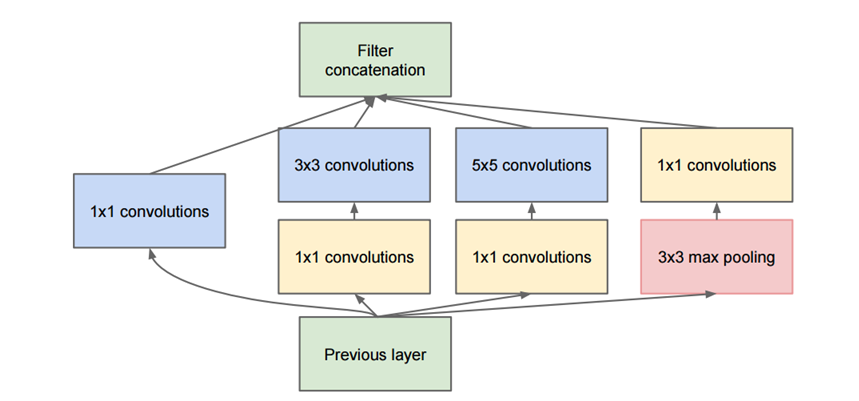
\includegraphics[scale=0.3]{./tex/convolution-network/classifier/inception.png}
    \caption{Architecture de l'Inception module}
    \label{inception}
\end{figure}

\noindent L'Inception module se démarque par la mise en parallèle de différentes couches de convolution appliquées sur une même source d'entrée dont les \textit{feature map} produites sont \textbf{concaténées} à la fin du bloc. Cette mise en parallèle des couches permet de créer différents \textit{flux} indépendants et différenciés les uns des autres. Chaque block peut avoir sa propre topologie, ce qui rend le modèle difficile à implémenter du fait de cette liberté. Évaluer la topologie d'un block est délicat et relève essentiellement de l'intuition. Il est important de relever la présence de convolution 1*1. Une approche naïve serait de les supprimer, leurs importances semblant être secondaires. Néanmoins, ce serait une erreur majeure. En effet, ces convolutions possèdent deux caractéristiques critiques dans le cadre de ce module:

\begin{itemize}
    \item \textbf{Réduction de dimension}: Les convolutions 1*1 possèdent la capacités de réguler la profondeur de la sortie d'une couche. Cette capacité est primordiale dans le cas de l'Inception module afin d'éviter une explosion inévitable de la dimension de sortie. Elle permettent ainsi de maîtriser la profondeur souhaitée d'une des branches du modules en sortie pour la concaténation (branche 3*3 max pooling) ou de diminuer la profondeur de la donnée d'entrée sur les branches 3*3 convolutions et 5*5 convolutions. En effet, l'application de filtre volumineux est gourmand en temps machine. Réduire la dimension de la donnée à observer favorise la vélocité du modèle. Les convolutions 1*1 permettent ainsi de réguler la dimension des données internes au module en maîtrisant les dimensions de sortie et en optimisant les dimensions de la données d'entrée pour favoriser un bon rapport performance/temps.

    \item \textbf{Non-linéarité}: Les convolutions 1*1 sont suivies d'une activation ReLu. De ce fait, elles permettent la mise en place de non-linéarité dans le module. Les couches de convolution étant linéaires dans leurs formes fondamentales, cet ajout ne peut être que bénéfique.
\end{itemize}

\noindent Cette architecture a eu plusieurs améliorations. La plus moderne est l'Inception-v4\cite{inceptionv4} qui propose une approche liant l'architecture Inception et Resnet.

\subsubsection{Xception}
Le modèle Xception\cite{xception}(2016) a été inventé par François Chollet, chercheur de Google à l'origine du framework \textit{Keras}. Xception propose une approche \textit{extrême} de l'approche \textit{Inception} d'où son appellation.\\

\noindent Afin de comprendre l'idée proposée par François Chollet, revenons sur le modèle Inception standard. Sur la Figure \ref{xception}, nous pouvons observer deux block Inception. A gauche, un block arbitraire (topologie variable) et à droite, un block simplifié avec une structure uniforme. Supposons un block de N flux. Par un jeu de manipulation, nous pouvons remplacer les N couches de convolution 1*1 indépendantes en une couche 1*1 unique de dimension N*P avec P profondeur des sorties des couches 1*1 indépendantes\footnote{On supposera les sorties uniformes}. Les \textit{feature map} de la couche 1*1 unitaire seront alors divisés en N parties sans chevauchement et alimenteront les différents flux de manière indépendante. Cette approche peut être poussée à \textit{l'extrême} en associant un flux à une unique \textit{feature map}. Une représentation graphique est visible sur la Figure \ref{xception2}. Le postulat du modèle Xception est une hypothèse plus forte que l'hypothèse d'Inception: il suppose que les corrélations inter-channels (profondeur) et les corrélations spatiales (largeur et longueur d'une \textit{feature map}) peuvent être complètement traitées séparément et non par sous-groupes.\\

\noindent Cette approche isolante est très similaire à une convolution Depthwise/Pointwise. Une différence majeure existe: une couche de Depthwise/Pointwise réalise une convolution standard pour créer les \textit{feature map} intermédiaires qui seront alors traitées par des convolutions 1*1. \textit{Extreme Inception} réalise exactement l'inverse. Les créateurs du modèle ne justifie pas concrètement le réel impact de cette inversion si ce n'est par leur intuition. De plus, dans un block Inception, une activation ReLu est appliquée entre les différentes couches afin d'appliquer de la non-linéarité, ce n'est pas le cas avec les couches Depthwie/Pointwise. Cette spécificité permet de mettre en avant un résultat remarquable. Alors que la non-linéarité est bénéfique dans le cas du block Inception standard\cite{inceptrelu}, elle semble être néfaste pour les blocks Extrem Inception avec Deptwise/Pointwise\cite{xception}. Ce résultat a été vérifié expérimentalement. Il est difficile de justifier clairement ce résultat mais l'idée principale repose sur la différence de profondeur. En effet, dans le block Inception standard, la profondeur de la données d'entrée dans un flux est profonde alors que dans un block Extrem Inception, la \textit{feature map} est unitaire. L'hypothèse est donc qu'appliquer une régularisation sur une donnée peu profonde provoque une perte d'informations trop importante.\\

\noindent La spécificité de la couche Depthwise/Pointwise permet ainsi de créer un réseau très simple d'implémentation. En effet, un block Extreme Inception n'est donc rien d'autre qu'une couche de Depthwise/Pointwise. L'architecture générale est standard et ne présente pas de particularité notable si ce n'est l'utilisation des \textit{résidus} (voir Section \ref{resnet} pour plus de détails sur cette notion).

\begin{figure}
    \centering
    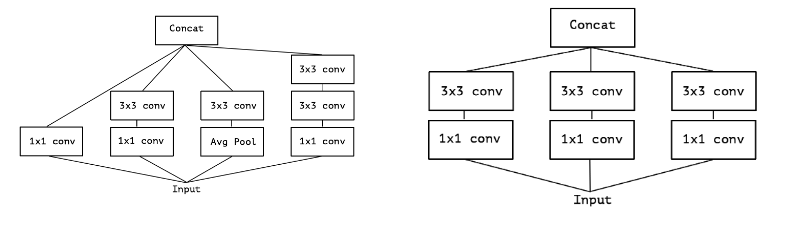
\includegraphics[scale=0.4]{./tex/convolution-network/classifier/xception.png}
    \caption{Architecture de l'architecture Xception: à gauche, un block standard et à droite un block simplifié (topologie uniforme)}
    \label{xception}
\end{figure}

\begin{figure}
    \centering
    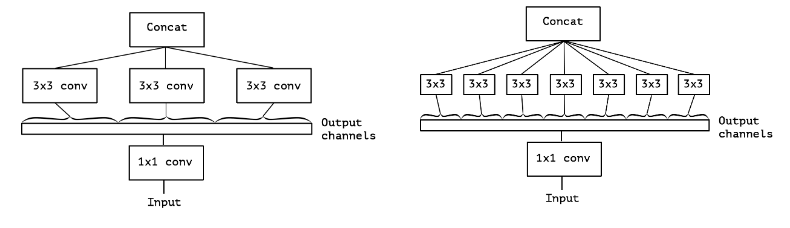
\includegraphics[scale=0.4]{./tex/convolution-network/classifier/xceptionv2.png}
    \caption{Architecture de l'architecture Xception: à gauche, un block Inception reformulé et à droite un block Inception dans sa forme extrême}
    \label{xception2}
\end{figure}

\subsubsection{Microsoft Resnet}
\label{resnet}

Resnet\cite{resnet}(2015) est le vainqueur de 2015 ILSVRC. Son taux d'erreur est exceptionnel (3,6\%). Un homme, en fonction de son expertise, obtient un taux d'erreur d'environ 5 à 10\%. Cette architecture est donc la première à faire significativement mieux que l'homme dans le cadre de cette compétition. Cette architecture repose sur le \textbf{Residual Block}. Une illustration est visible sur la figure \ref{residual}.\\

\begin{figure}
    \centering
    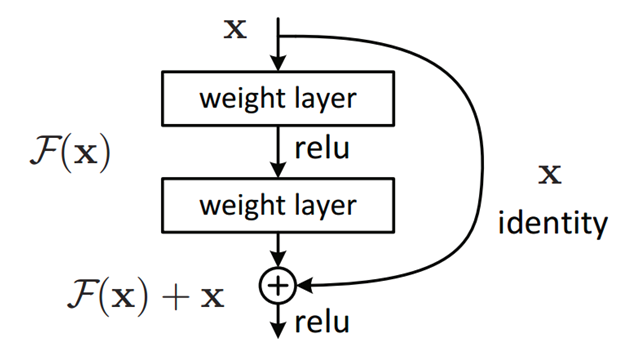
\includegraphics[scale=0.3]{./tex/convolution-network/classifier/residual.png}
    \caption{Architecture du Residual Block}
    \label{residual}
\end{figure}

\noindent Un \textit{Residual Block} est caractérisé par la non-perte de la donnée d'entrée. Ainsi, la sortie de ce block calcule un changement de faible ampleur (un "Delta") afin d'obtenir une version légèrement altérée de la donnée d'entrée. Pour conserver la donnée d'entrée, une concaténation est réalisée à la sortie du block où la sortie des couches internes est \textbf{additionnée}\footnote{Au sens strict du terme, non concatenée} à la donnée d'entrée\footnote{En cas de dimension différente entre l'entrée et la sortie des couches internes du bloc, du 0-padding et/ou des convolutions 1*1 sont utilisées}. Cette architecture favorise un bon apprentissage en facilitant la propagation d'un gradient "valide", notamment en luttant contre le problème de \textit{vanishing gradient}. L'idée derrière la notion de \textit{Résidus} est qu'il est plus facile d'approximer une fonction qui nullifie les résidus plutôt que d'approximer une fonction identité (Figure \ref{residual2}) . Néanmoins, son efficacité théorique n'est pas démontrée malgré une efficacité empirique et expérimentale incontestable.\\

\begin{figure}
    \centering
    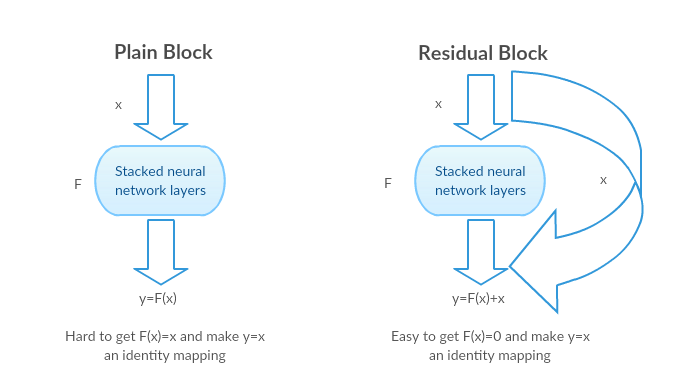
\includegraphics[scale=0.3]{./tex/convolution-network/classifier/resnet2.png}
    \caption{Intuition sur la notion de Résidus}
    \label{residual2}
\end{figure}

\noindent \textbf{Important}: Les architectures \textit{state-of-the-art} reposent essentiellement sur ce type d'architecture\footnote{Plusieurs architectures peuvent être cumulées !}. Il est souvent pertinent de considérer ce type de réseau convolutif lorsqu'un choix par défaut s'impose.

\subsubsection{ResNet et améliorations}
Du fait de l'efficacité des réseaux Resnet, la recherche est active autour de cette architecture. Plusieurs améliorations ont été proposées: \\

\paragraph{Wide Residual Network}

\noindent Wide Residual Network\cite{wideres}(2016) propose une architecture qui s'étend en "largeur"\footnote{Ne pas confondre ! Il y a une augmentation sur un unique flux de couches (ajout de filtres ou d'un DropOut par exemple) uniquement. L'augmentation se fait en largeur car elle ajoute des entités sur une couche ciblée au sein d'un même flux, non en largeur avec l'ajout de flux parallèles comme les modèles Inception !} et non uniquement en profondeur comme l'approche initiale des ResNets. La démarche principale consiste augmenter le nombre de filtres par couche ou implanter des couches spécifiques (dropout, 1*1 convolution,...). Ainsi, cette architecture crée plus de \textit{feature map} en interne et possède un plus fort pouvoir de discrimination. Néanmoins, il peut y avoir une hausse du nombre de paramètres donc un temps de calculs et d'apprentissage supérieurs. Pour s'opposer à ce problème, la profondeur est minorée par rapport à la largeur. De plus, les capacités de calculs sont optimisées avec les approches en largeur car le calcul des différentes \textit{feature map} au sein d'une même couche est fortement parallélisable, ce qui favorise la vélocité du modèle. Cette architecture propose aussi l'ajout de DropOut ou de convolutions 1*1 à l'intérieur des blocs. La plus-value de cet article est de montrer qu'un réseau ResNet ne doit pas être que profond mais favoriser son expansion en largeur aussi. Une illustration de cette architecture est représentée sur la Figure \ref{wide}.

\begin{figure}
    \centering
    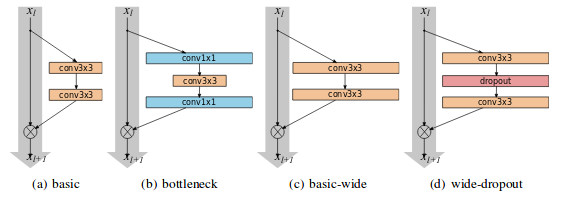
\includegraphics[scale=0.4]{./tex/convolution-network/classifier/wideresnet.png}
    \caption{Architecture d'un Wide Residual block (les étapes de Batch normaliszation) et de ReLu ne sont pas affichées) - la largeur des rectangles représentant les couches déterminent graphiquement le nombre de filtres employés pour la couche associée}
    \label{wide}
\end{figure}

\paragraph{Aggregated Residual Transformations for Deep Neural Networks (ResNext)}

\noindent Le réseau ResNext\cite{resnext}(2016) est le modèle arrivé 2nd au 2016 ILSVRC. Cette architecture propose de lier les caractéristiques des modèles ResNet et Inception. La principale caractéristique de ResNext repose sur son expansion en largeur avec l'ajout de flux internes dans un block. Sa différentiation majeure avec l'approche d'Inception est l'utilisation d'une topologie de bloc identique pour chaque bloc. La différenciation des blocks se fait au niveau du facteur de profondeur qui détermine le nombre de flux parallèles au sein d'un block.\\

\noindent L'architecture Resnext propose trois formes de blocks équivalents pour structurer son réseau.

\begin{itemize}
    \item \textbf{Approche ResNet}: Avec cette approche, chaque flux réalise une harmonisation de la dimension indépendamment des autres flux via une convolution 1*1. Les \textit{feature map} issues des différents flux du block sont additionnées. La sortie est alors additionnée avec l'entrée du block.

    \item \textbf{Approche Inception}: Avec cette approche, l'harmonisation de la dimension est mutualisée. Ainsi, l'ensemble des \textit{feature map} issues des flux sont concaténées sans application de convolution 1*1 et produisent une sortie intermédiaire. L'application de la convolution 1*1 est réalisée sur la sortie intermédiaire et les \textit{feature map} obtenues sont additionnées à l'entrée du block.

    \item \textbf{Approche par convolution groupée}: Cette approche repose sur l'implémentation du réseau AlexNet qui a groupé ses couches afin de paralléliser son réseau sur différents GPU. Resnext propose cette méthode en considérant un flux comme un groupe. Ils peuvent donc être partagés sur différents GPU et favoriser la vélocité du modèle. Cette représentation est essentiellement théorique et peu exploitée dans les faits.
\end{itemize}

\noindent Une représentation graphique des différentes architectures du block ResNext est visible sur la Figure \ref{resnext}.

\begin{figure}
    \centering
    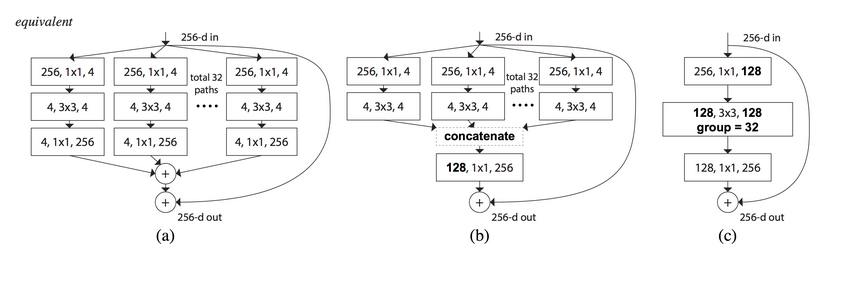
\includegraphics[scale=0.4]{./tex/convolution-network/classifier/resnext.png}
    \caption{Différentes représentations de l'architecture d'un block du réseau ResNext: 1) Approche ResNet, 2) Approche Inception, 3) Approche par convolution groupée}
    \label{resnext}
\end{figure}

\paragraph{Densely Connected Convolutionnal Networks (DenseNet)}

\noindent Densely Connected Convolutionnal Networks\cite{densely}(2016) généralise la transmission de l'entrée des blocs ResNet en projetant l'entrée d'une convolution sur l'ensemble des convolutions suivantes et non juste le suivant direct. Ainsi, la $n^{ieme}$ couche possédera une entrée issue de n sources. De même, la $n^{ieme}$ couche transmettra sa sortie aux (N-n) couches suivantes avec N, nombre total de couche. Il y a donc $\frac{N(N+1)}{2}$\footnote{Équivalent à la somme de 1 à n} connexions dans l'ensemble du réseaux issues des divers blocs au lieu de N d'où le nom de \textit{Densely connected}. De plus, l'entrée est \textbf{concaténée} et non additionnée comme dans un bloc ResNet standard. La concaténation implique une augmentation constante de la profondeur de l'entrée transférée à chaque bloc. L'ajout de convolution 1*1 et de pooling est donc une nécessité pour éviter l'explosion du nombre de données en entrée. Veuillez vous référer à l'article \cite{densely} pour plus de détails sur cette régulation. \\

\noindent Le réseau DenseNet, visible sur la Figure \ref{DenseNet}, est composé de plusieurs Dense block séparés par un block de transition formé d'une convolution 1*1 et d'un Pooling afin de redimensionner les \textit{feature map}. Ce redimensionnement pose problème car les \textit{feature map} des block précédents ne sont plus de même dimension que les block qui suivent. De ce fait, la propagation se limite à un Dense block et non à l'ensemble du réseau.

\noindent La conversion de l'addition vers la concaténation apporte une plus-value importante. La concaténation préserve la structure de la \textit{feature map} peu importe l'éloignement du bloc par rapport au bloc considéré. Cette différence permet de s'opposer au problème de corruption de l'information transférée ou de son effacement qui augmente alors que le nombre de \textit{feature map} additionnées augmente linéairement. De plus, le modèle peut apprendre une combinaison optimal entre les features map concatenées, ce qui permet une meilleure interprétation de l'information utile. \\

\noindent Bien que paradoxale, cette approche permet de limiter le nombre de paramètres nécessaire pour créer le modèle. Dans un réseau neuronal, chaque couche lit une entrée donnée par la couche précédente associée et écrit à la couche suivante. La couche actuelle modifie donc l'état mais transmet aussi l'information importante à conserver. Cette information est conservée, dans les réseaux ResNet, par addition avec l'identité de l'entrée. Cependant, il a été montré que certaines couches contribuent peu voire produisent de l'information redondante (il se peut qu'elles redéfinissent une information perdues déjà calculée précédemment dans le modèle) et donc, peuvent être supprimées. Afin de considérer cette particularité, la structure Densely connected propose une meilleure mémoire de la donnée utile et des modifications réalisées en projetant l'information sur l'ensemble des blocs et non uniquement le suivant. Cette propagation (et conservation) de l'information permet de limiter grandement le nombre de couches/blocs et ainsi de limiter le nombre de paramètres, rendant le modèle plus léger et rapide à apprendre. L'intuition derrière cette idée peut être contre-intuitive. Pour une explication détaillée, veuillez vous référer à l'article associé \cite{densely}. La structure d'un réseau Densely Connected est visible sur la Figure \ref{densely}.\\

\begin{figure}
    \centering
    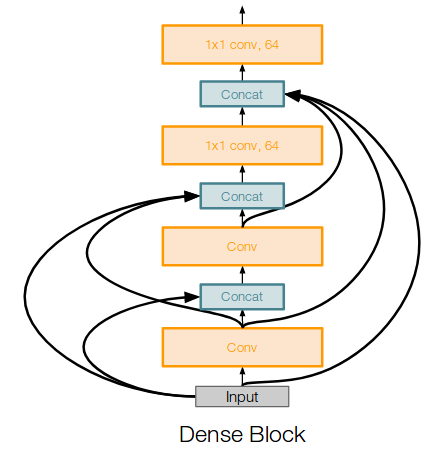
\includegraphics[scale=0.4]{./tex/convolution-network/classifier/dense.png}
    \caption{Architecture d'un réseau Densely Connected}
    \label{densely}
\end{figure}


\begin{figure}
\hspace{-3cm}
    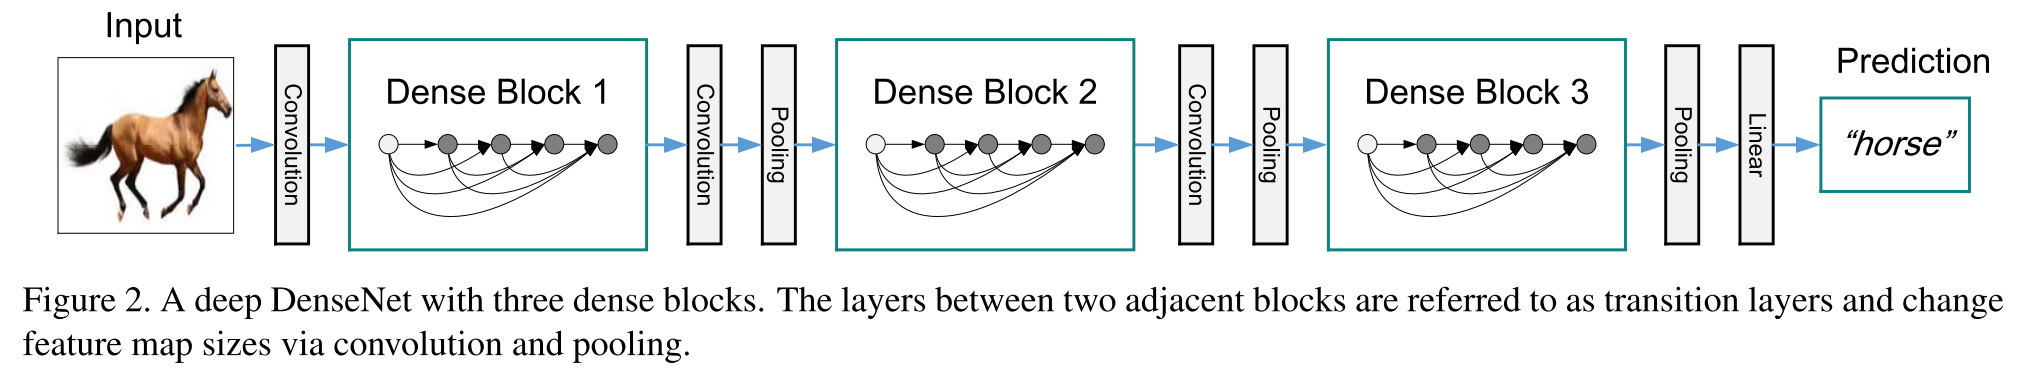
\includegraphics[scale=0.25]{./tex/convolution-network/classifier/densenet.png}
    \caption{Réseau DenseNet}
    \label{DenseNet}
\end{figure}

\paragraph{Stochastic Depth}

\noindent Stochastic Depth\cite{stores}(2016) met en relation le DropOut et les spécificités des \textit{Résidual block} des réseaux résiduels. Afin de limiter l'inter-dépendance des couches du réseaux, les blocks sont conservés (sinon ils sont équivalents à une couche \textit{identité}) selon une probabilité $p_l$. $p_l$ est une probabilité constante (peu optimale) ou linéaire dégressive telle que $p_l=1-\frac{l}{L}*(1-p_L)$ (par défault, $p_L$ est égal à 0.5 et correspond à la valeur limite du dernier block considéré dans le réseau) avec L, nombre total de block et l, le block ciblé. Comme pour le DropOut, durant la phase de test, chaque sortie de residual block (avant union avec la valeur d'entrée du bloc) est active et pondérée selon la valeur du pourcentage d'activation associée. Un exemple illustratif est visible sur la Figure \ref{stores_fig}.

\begin{figure}
    \centering
    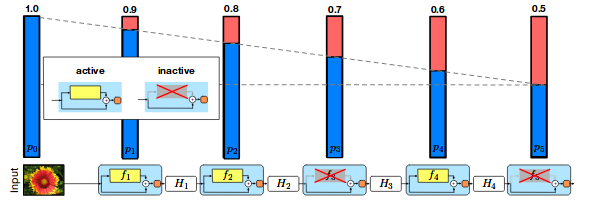
\includegraphics[scale=0.4]{./tex/convolution-network/classifier/stores.png}
    \caption{Stochastic Depth routine}
    \label{stores_fig}
\end{figure}

\paragraph{Residual Networks of Residual Networks: Multilevel Residual Networks}

Residual Networks of Residual Networks\cite{RoR}(2016) propose une approche basée sur la structure de groupe. Ainsi, le réseau est composé d'une succession de groupes composés de block à la structure similaire. Le créateur du modèle a utilisé des convolutions 3*3 uniquement de profondeur variable appartenant à $[16,32,64]$. Trois groupes est donc formés en fonction de la largeur des couches. Il n'y a pas d'intersection de groupe, i.e chaque groupe est unique et els groupes sont homogènes. Supposons un réseau avec N block alors un groupe possèdera $\frac{N}{3}$ block. Ce réseau se différencie du ResNet en ajoutant une connexion inter-block pour chaque groupe. Ainsi, les \textit{feature map} en entrée du premier block d'un groupe seront additionnées aux \textit{feature map} de sortie de ce groupe. Un exemple de ce réseau est visible sur la Figure \ref{ror}.\\

\noindent La notion de groupe est variable selon le niveau de coupure P choisi. Ainsi, pour P=1, on considère un groupe uniquement. Le réseau est donc semblable à un ResNet standard (pas de liaison inter-groupe). Pour P=2, on considère 2 groupes. Ainsi, la connexion inter-block est unique et relie l'entrée du premier bloc avec la sortie du dernier bloc du réseau. De même, pour P=3, on considère 3 niveaux de groupe. De ce fait, une connexion inter-block est faite entre le premier et dernier block de même largeur de couche (16,32 ou 64 dans le cas présent). \\

\noindent L'architecture du modèle est généraliste et peut être associée à des modèles existants tels que Wide Residual Network par exemple. L'idée portée par l'auteur est de ne pas se limiter à la connexion entre un block et son successeur mais réaliser une connexion entre l'entrée et la sortie d'un \textit{Super-Block} composé d'un ensemble de block de même nature. Cette approche propose ainsi une approche dépendante de l'architecture de groupe de réseau alors que l'approche Densely conencted et Sparsely Connected considère le block de manière unitaire et isolée.

\begin{figure}
    \centering
    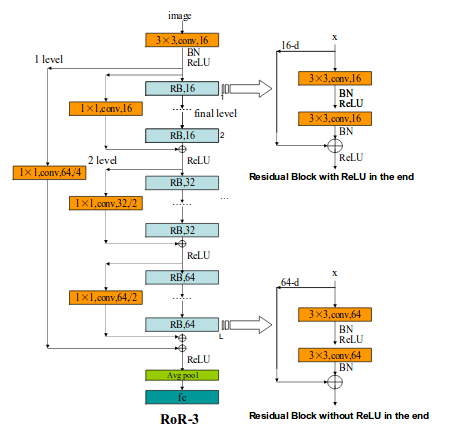
\includegraphics[scale=0.4]{./tex/convolution-network/classifier/ror.png}
    \caption{Exemple d'un réseau RoR de niveau 3}
    \label{ror}
\end{figure}

\paragraph{Sparsely Connected Convolutional Networks (SparseNet)}

Sparsely Connected Convolutional Networks\cite{sparsenet}(2018) repose sur les fondations du réseau DenseNet à la différence que les sorties des blocks ne sont pas transmises à l'ensemble des couches suivantes mais en fonction d'un offset exponentiel. En effet, pour un block $B_n$, seules les sorties des couches $B_{n-1}, B_{n-2},B_{n-4}, B_{n-8},...,B_{n-2^k}$ avec k, plus grand entier non négatif tel que $2^k<l$, sont considérées. Une comparaison entre SparseNet et DenseNet est visible sur la Figure \ref{sparsenet}.\\

\noindent L'approche par concaténation proposée par DenseNet a permis une amélioration significative du modèle ResNet en corrigeant le défaut de la méthode additive. Néanmoins, cette approche pose un problème du fait de l'explosion du nombre de connexions qui est de complexité $O(N^2)$. Cette augmentation de paramètres présente un risque d'overfitting et une explosion de la consommation mémoire du réseau lorsqu'il est profond. De plus, diverses expériences ont montré que l'utilisation de l'information transmise par les connexions inter-block est mal exploitée par le réseau avec une part importante de \textit{feature map} transférées sans réel pouvoir explicatif. Le réseau DenseNet est donc \text{trop} dense. L'ajout d'un offset exponentiel d'ordre 2 permet ainsi de limiter ce défaut en limitant la complexité à $O(log(n))$\footnote{On peut grossièrement considérer que le nombre de connexions inter-block total est borné du fait de la faible croissance de la fonction logarithme} tout en conservant l'information utile portée par les différentes connexions inter-block. l'hypothèse est faite qu'il est préférable de privilégier l'information portée par les block adjacents que les block très éloignés.


\begin{figure}
    \centering
    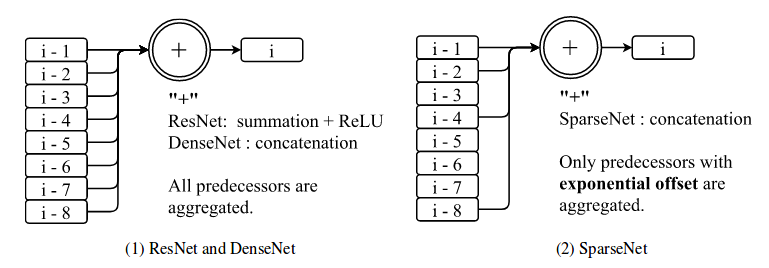
\includegraphics[scale=0.4]{./tex/convolution-network/classifier/sparsenet.png}
    \caption{Différence entre un block issu de ResNet, DenseNet et SparseNet}
    \label{sparsenet}
\end{figure}

\paragraph{Résumé des différentes approches appliquées aux ResNet}

Ci-dessous, un tableau récapitulatif de l'ensemble des améliorations étudiées concernant les réseaux ResNet. Certaines de ces méthodes sont cumulatives. Approfondir leurs interactions est une piste de recherche intéressante et pertinente.\\

\hspace{-2.5cm}\begin{tabular}{|c|c|}
 \hline
  Méthodes & Spécificités\\
  \hline
  Wide Residual & Elargissement du flux d'un bloc\\
  & Utilisation de couches spécifiques (DropOut...)\\
  \hline
  Aggregated Residual Transformations & Ajout de flux dans un block \\
  \hline
  Densely Connected &  Propagation de la sortie sur l'ensemble des couches suivantes\\
  & Concaténation de la sortie du block avec son entrée\\
  \hline
  Residual Networks of Residual Networks & Propagation de la sortie selon les groupes de block\\
  \hline
  Sparsely Connected & Propagation de la sortie selon un offset exponentiel\\
  & Concaténation de la sortie du block avec son entrée\\
  \hline
  Stochastic Depth & Non-utilisation de block durant l'apprentissage (probabiliste)\\
  \hline
  Squeeze-and-Excitation & Pondération des \textit{feature map}\\
  \hline
\end{tabular}

\subsubsection{FractalNet: Ultra-Deep Neural Networks without Residuals}
Le modèle FractalNet\cite{fractalnet}(2016) est une approche qui s'émancipe de l'architecture des ResNet (ou dérivés) et se présente comme une alternative viable. Ce réseau démontre que, bien que très efficace, l'approche par résidu n'est pas la seule approche compétitive et performante. Néanmoins, FractalNet est un réseau récent encore méconnu. Il est donc difficile de juger pleinement de ses capacités. La structure du réseau Fractalnet est comparable au comportement d'une fractale, i.e la structure du réseau suit un modèle similaire peu importe le sous-réseau observé. La structure fondamentale du ce réseau est explicitée par la Figure \ref{fractalnet}.\\

\noindent FractalNet exploite une alternative au DropOut afin de régulariser son réseau. Le processus, appelé \textbf{Drop-path} se divise en deux parties:

\begin{itemize}
    \item \textbf{Local}: L'étape Local désactive des flux (ou entrées de couche \textit{join}) aléatoirement selon une probabilité fixée. Il y a une garantie de l'existence d'au moins un flux pour chaque couche \textit{join}.

    \item \textbf{Global}: L'étape Global sélectionne un unique path pour tout le réseau et désactive tous les autres flux. Cette approche permet de limiter les dépendances entre flux, de masquer l'origine du flux et ainsi, de bloquer le comportement du réseau qui viserait à considérer un flux comme un résidu ou un terme correctif.
\end{itemize}

\noindent La couche \textit{join} peut sembler similaire à l'additivité employée dans un réseau ResNet. Cependant, il existe des différences critiques non négligeables:

\begin{itemize}
    \item \textbf{Non différenciation de la source}: Contrairement au réseau ResNet, le réseau FractalNet ne différencie pas le flux associé à un résidu et le flux associé à la couche interne du block. Cette non-différentiation est permise grâce au transfert direct sans transformation préalable à la couche de convolution suivante.

    \item \textbf{Régularisation par Drop-path}: Ce procédé permet de forcer chaque flux à être \textit{viable}. De ce fait, la régularisation favorise un apprentissage qui punit les flux qui évoluent vers un comportement de \textit{résidu}.

    \item \textbf{Sous-réseau unitaire et performant}: Le Drop-path, du fait de son étape \textit{Global} favorise les performances de sous-réseaux unitaires, i.e qui n'exploite pas les caractéristiques de la couche \textit{join}. En effet, l'étape \textit{Global} force les couches \textit{join} à n'avoir qu'une seule entrée. Ainsi, ces sous-réseaux sont fonctionnels et produisent un signal qui ne devrait pas "recevoir" de résidu pour être efficace.
\end{itemize}

\begin{figure}
    \centering
    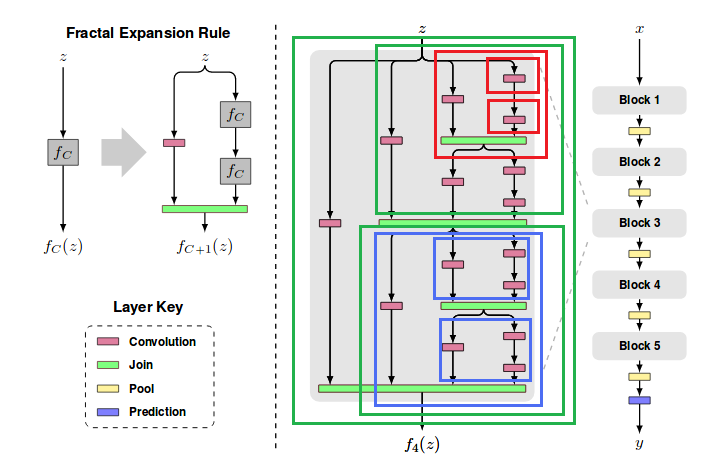
\includegraphics[scale=0.4]{./tex/convolution-network/classifier/fractalnet.png}
    \caption{Construction d'un bloc du réseau FractalNet}
    \label{fractalnet}
\end{figure}

\subsubsection{Classement des architectures standards}
Le graphique présent sur la Figure \ref{ranking} résume les caractéristiques des différentes architectures vues précédemment. Ainsi, en résumé, nous pouvons observer que SENet et NASNet font office d'état de l'art actuellement en terme de performances brutes. On peut observer la domination de NASNet sur ses concurrents pour chaque catégorie de modèle (léger/intermédiaire/lourd). Néanmoins, NASNet est critiqué pour son architecture qui présenterait des difficultés à être efficace sur des jeux de données autres que ImageNet ou CIFAR, contrairement à SENet ou des modèles standards reposant sur des architectures Inception ou ResNet. Les modèles VGG sont très lourds, lents et avec une efficacité en déclin bien que toujours très employés comme extracteur d'attribut dans le cadre d'architectures complexes. Tout comme AlexNet, ils tendent à devenir obsolètes. Pour une étude complète et détaillée des différents modèles de Deep Learning, veuillez vous référer à l'article \cite{ranking2}\footnote{Étant donné la rapide évolution des modèles convolutifs, cette étude peut être obsolète lors de votre lecture.}.\\

\noindent \textbf{Remarque}: NASNet est une architecture qui a été crée par un générateur automatique (dévellopé par Google) selon l'algorithme \textit{Neural Architecture Search} qui exploite l'apprentissage par renforcement. Il s'agit donc d'une architecture entièrement crée indépendamment de l'Homme. A la vue de ses performances, il est possible qu'à l'avenir, l'optimisation d'architecture neuronale se fasse grâce à des algorithmes automatiques.

\begin{figure}
    \centering
    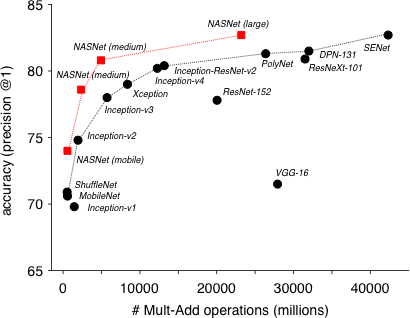
\includegraphics[scale=0.45]{./tex/convolution-network/classifier/nasnet.jpg}
    \caption{Analyse des réseaux de Deep Learning (2018)}
    \label{ranking}
\end{figure}

\subsubsection{Réseaux de neurones compressés}

Les modèles étudiés précédemment sont pour la plupart gourmands et lourds. Ils posent un problème de mémoire et de performance sur des supports de faible capacité comme l'embarqué ou les appareils nomades tels que les smartphones. Afin de répondre à cette problématique, une optimisation du temps de calculs et du nombre de paramètres sont nécessaires tout en limitant la perte de la qualité prédictive du réseau. Ce type de réseaux dits \textit{compressés} ont une importance élevée du fait de leurs capacités de commercialisation notamment à travers les applications des supports mobiles (téléphones, tablettes, domotiques...)

\paragraph{SqueezeNet}
\label{squeezesect}
Le réseau SqueezeNet\cite{squeezenet}(2016) est un réseau développé pour être supporté par les supports les plus \textit{faibles}. Sa structure cherche donc à limiter le nombre de paramètres et son impact mémoire. Ainsi, par rapport à AlexNet (qui lui sert de référence), SqueezeNet est 50x plus léger et son poids peut être 510x plus faible avec application de méthode de compression de réseau, notamment Deep Compression (voir Section \ref{deepcompsec}). Sans compression, ce réseau pèse 4.8MB et après compression, 0.47. Cette taille minime lui permet d'être implémenter sur de nombreuses structures de faible capacité bien que la précision du réseau soit significativement inférieure aux autres réseaux (bien plus volumineux). Il reste cependant satisfaisant pour des tâches de faible complexité ou sans nécessité de précision de haute performance.\\

\noindent La structure de ce réseau repose sur trois principes:

\begin{itemize}
    \item \textbf{Utilisation en majorité de filtre 1*1 à la place de 3*3} afin de limiter le nombre de paramètres à apprendre et le nombre de calculs nécessaires.

    \item \textbf{Diminution du nombre de channels entrants dans une couche de convolution}. Cette diminution est réalisée grâce à une couche \textit{squeeze}\footnote{Nous verrons par la suite la configuration de cette couche}. Afin de ne pas trop perturber la précision du modèle en supprimant en excès les filtres 3*3, limiter le nombre de channels à analyser est une alternative efficace. En effet, le nombre de calculs à réaliser pour une couche de convolution 3*3 est: $nbr_{inputChannel}*nbr_{filtre}*(3*3)$.

    \item \textbf{Conservation de la dimension de l'entrée} afin de favoriser une bonne précision du modèle. En effet, les principes précédents favorisent une réduction du poids du réseau au détriment de sa performance. Il est donc nécessaire de lutter contre une trop grande détérioration de la précision. Pour cela, la dimension des \textit{\textit{feature map}} est faiblement modifié jusqu'en fin de réseau contrairement à la plupart des réseaux plus volumineux qui réalisent de nombreuses transformations internes, notamment via l'application d'un stride supérieur à 1 ou des approches par \textit{Pooling}. Cette idée relève d'une intuition des créateurs du réseau et n'a pas de preuve véritablement démontrée.
\end{itemize}

\noindent Afin de respecter les deux premiers principes, un nouveau type de block est crée: le \textit{Fire Module}. Ce module est séparé en deux parties: la partie \textit{Squeeze} et la partie \textit{expand}. La partie Squeeze est uniquement composée de filtres 1*1 (Principe 1), la partie Expand analyse les \textit{\textit{feature map}} issues de la partie Squeeze et est composée de filtres 1*1 et 3*3. Le nombre de filtre 1*1 dans la partie Squeeze est inférieur au nombre de filtres (1*1 et 3*3) dans la couche Expand, ce qui permet de maîtriser la profondeur des entrées et de conserver un nombre de dimension restreint sans négliger le nombre de filtre (Principe 2). L'absence de \textit{Pooling} et de stride permet de garder les mêmes dimension de \textit{feature map} (hauteur et largeur). Le block possède de nombreux hyperparamètres afin de définir la répartition des filtres et l'évolution de la configuration du filtre au fil du réseau. Pour plus de détails, veuillez consulter l'article\cite{squeezenet}. Une illustration du block est visible sur la Figure \ref{firemodule}.\\

\noindent L'architecture du réseau repose sur une succession de Fire Module régulièrement régulée par des couches de pooling inter-block. Il est intéressant de noter que le nombre de \textit{feature map} de sortie augmente régulièrement jusqu'à la fin du réseau, ce qui traduit une augmentation du nombre de filtres. De plus, ce réseau possède une architecture standard ou résiduelle. Dans le cas d'une architecture résiduelle, deux approches sont possibles. La première consiste à réaliser une connexion interblock à chaque fois que la dimension de l'entrée est identique à la dimension de sortie (\textit{simple bypass}). La seconde crée une connexion interblock pour chaque bloc. En cas de différence de dimensions, une couche de convolution 1*1 mettra à l'échelle la profondeur du résidu du block considéré (\textit{complex bypass}). L'ajout de la structure résiduelle sert à palier la perte d'informations associée à la couche \textit{Squeeze} des blocs.

\begin{figure}
    \centering
    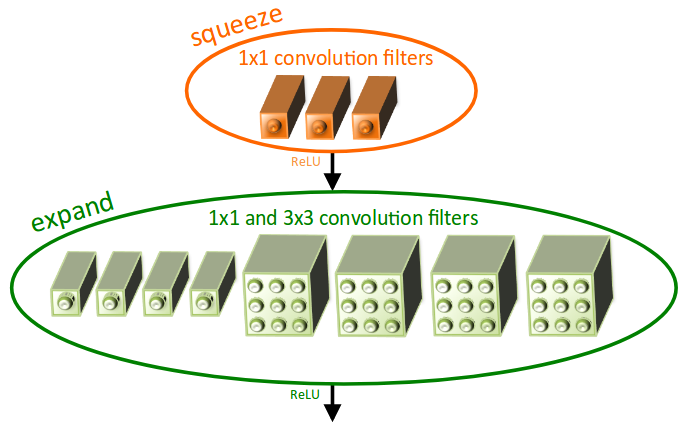
\includegraphics[scale=0.4]{./tex/convolution-network/classifier/squeezbloc.png}
    \caption{Architecture du Fire Module}
    \label{firemodule}
\end{figure}

\paragraph{MobileNet}

L'une des architectures les plus populaires est MobileNet\cite{mobilenet}(2017). Ce modèle exploite les convolutions Depthwise/Pointwise afin de limiter son impact mémoire et accélérer sa vélocité. Les filtres des Depthwise sont de taille 3*3 uniquement, ce qui est un standard avec le filtre 5*5. Cette dimension de filtre reste néanmoins l'un voire le meilleur rapport temps/précision/mémoire pour un modèle qui se veut léger et rapide. \\

\noindent L'architecture se veut modulable et adaptatif. Pour cela, deux hyperparamètres ont été instaurés: le \textbf{multiplicateur de largeur} et le \textbf{multiplicateur de résolution}. Ces paramètres de modifier la structure du réseau tout en conservant son intégrité et sa structure, uniforme. Il est donc possible de paramétrer aisément sa profondeur afin de l'adapter aux différentes capacités des supports d'application.

\begin{itemize}
    \item \textbf{Multiplicateur de largeur}: Ce critère (noté $\alpha$) joue sur la profondeur des entrées et des sorties des couches de convolutions en adaptant leurs dimensions selon un coefficient. Ainsi, en reprenant les résultats obtenus dans la Section \ref{depthwiseconv}, nous obtenons: $$D_{depthwise/poitnwise, \alpha}=(X*X)*\alpha M*(K*K)*1+(X*X)*\alpha M*(1*1)*\alpha N$$

    En pratique, cet hyperparamètre est implémenté de manière à limiter le nombre de \textit{feature map} de sortie d'une couche de convolution. En effet, cette sortie sera l'entrée de la couche suivante. Il est donc évident que si la dimension d'une sortie est minorée, la dimension de l'entrée de la couche suivante le sera aussi.

    \item \textbf{Multiplicateur de résolution}: Ce critère (noté $\rho$) modifie la dimension de l'image d'entrée, réduisant ainsi la représentation interne dans chaque couche du réseau. Nous obtenons ainsi:
    $$D_{depthwise/pointwise, \rho}=(\rho X*\rho X)*M*(K*K)*1+(\rho X*\rho X)*M*(1*1)*N$$

    Ce critère est peu explicité dans l'article publié et son implémentation douteuse. Il est possible qu'il soit théorique et au final, non représenté concrètement.
\end{itemize}

\noindent Avec l'application des deux coefficients, l'équation du coût de ce réseau s'exprime donc sous la forme:
$$D_{depthwise/poitnwise,\alpha,\rho}=(\rho X*\rho X)*\alpha M*(K*K)*1+(\rho X*\rho X)*\alpha M*(1*1)*\alpha N$$

\paragraph{Modèles expérimentaux récents}

Afin d'approfondir l'état de l'art, voici une liste de modèles récents prometteurs qu'il peut être intéressant d'étudier:

\begin{itemize}
    \item ShuffleNet\cite{shufflenet} (Dec 2017): Architecture pour support de faible puissance (smartphone par exemple). Ses résultats semblent meilleurs que MobileNet pour un coût machine plus faible.
    \item EffNet\cite{effnet} (En cours d'écriture - Mars 2018): Architecture pour support de faible puissance (smartphone par exemple). Plus récent que MobileNet et ShuffleNet, il cherche à corriger leurs défauts. En cours d'écriture, il n'est pas possible de juger les résultats de cette architecture actuellement mais les résultats intermédiaires sont prometteurs.
\end{itemize}

\subsubsection{Les jeux de données de référence}
Le Deep Learning nécessitant de nombreuses données, la création de jeux de données de qualité a été au coeur de la Recherche. Bien que ce soit encore une thématique en cours d'étude, de nombreux jeux de données ont été crées pour effectuer des \textit{benchmarks} compétitifs, répondre à une problématique ou tout simplement, faciliter le développement des algorithmes de Deep Learning en soulageant la difficulté de création d'un jeu de données. \\

\noindent L'analyse d'image étant le secteur historique principal du Deep Learning, de nombreux jeux de données ont été crées. Il est intéressant d'en connaître les principaux afin de pouvoir les utiliser dans des projets. Dans cette section, nous allons considérer les jeux de données concernant l'analyse d'image uniquement.
\begin{itemize}
    \item \textbf{MNIST: handwritten digits}\cite{mnist}: Ce jeu de données est historique et a accompagné l'ascension des réseaux convolutifs. Il est constitué de chiffres entre 0 et 9 écrit à la main représentée en noir et blanc\footnote{Des variantes ont été crées en niveau de gris}. Souvent utilisé pour évaluer la pertinence d'un modèle, il tend à devenir obsolète car trop "facile" à résoudre. Les meilleurs modèles actuels dépassent 99\% sur ce jeu de données.
    \item \textbf{CIFAR10 / CIFAR100}\cite{cifar10}\cite{cifar100}: Il s'agit d'un jeu de données généraliste composé d'image 32*32 réparties en 10/100 classes. Il n'est pas très utilisé mais permet d'évaluer les performances d'un modèle de manière préventive avant d'exploiter des jeux de données plus populaires et plus "exigeants".
    \item \textbf{Pascal VOC}\cite{pascal}: Ce jeu de données est relativement ancien et n'est plus mis à jour. Il est rarement utilisé dans le cadre d'apprentissage pour de la classification d'image mais très populaire pour la détection d'objet.
    \item \textbf{ImageNet}\cite{imagenet}: C'est l'un des jeu de données les plus riches actuellement. Avec plus de 10 millions d'image pour 1000 catégories, il offre une richesse d'apprentissage de premier ordre. Une partie de ce jeu de données a été convertie en \textit{bounding boxes}. Avec de nombreuses API disponibles, ce jeu de données a l'ambition de devenir une voire la référence pour l'apprentissage générique. Il est associé à une compétition annuelle (ILSVRC) qui est considérée comme l'une voire la compétition la plus prestigieuse en analyse d'image actuellement.
    \item\textbf{MS COCO}\cite{coco}: Il s'agit d'un jeu de données générique (2.5 millions d'image pour 91 classes) associé à une compétition d'analyse d'image (COCO). Étant légèrement dans l'ombre d'ImageNet en terme de popularité, ce jeu de données s'illustre avec ses images annotées (\textit{captioning}).
\end{itemize}

\noindent Ces jeux de données sont les références \textit{généralistes}. Il existe de nombreux autres jeux de données généralistes tout comme des spécialisés, notamment d'images de visage (pour la reconnaissance faciale), des images aériennes/satellites ou encore des images issues de la \textit{Physique} (astrophysique/cosmologie, physique fondamentale, mécanique...) et de la Médecine/Biologie (imagerie médicale) par exemple.
